% Options for packages loaded elsewhere
% Options for packages loaded elsewhere
\PassOptionsToPackage{unicode}{hyperref}
\PassOptionsToPackage{hyphens}{url}
%
\documentclass[
  ignorenonframetext,
  aspectratio=169,
  spanish,
  professionalfonts]{beamer}
\newif\ifbibliography
\usepackage{pgfpages}
\setbeamertemplate{caption}[numbered]
\setbeamertemplate{caption label separator}{: }
\setbeamercolor{caption name}{fg=normal text.fg}
\beamertemplatenavigationsymbolsempty
% remove section numbering
\setbeamertemplate{part page}{
  \centering
  \begin{beamercolorbox}[sep=16pt,center]{part title}
    \usebeamerfont{part title}\insertpart\par
  \end{beamercolorbox}
}
\setbeamertemplate{section page}{
  \centering
  \begin{beamercolorbox}[sep=12pt,center]{section title}
    \usebeamerfont{section title}\insertsection\par
  \end{beamercolorbox}
}
\setbeamertemplate{subsection page}{
  \centering
  \begin{beamercolorbox}[sep=8pt,center]{subsection title}
    \usebeamerfont{subsection title}\insertsubsection\par
  \end{beamercolorbox}
}
% Prevent slide breaks in the middle of a paragraph
\widowpenalties 1 10000
\raggedbottom
\AtBeginPart{
  \frame{\partpage}
}
\AtBeginSection{
  \ifbibliography
  \else
    \frame{\sectionpage}
  \fi
}
\AtBeginSubsection{
  \frame{\subsectionpage}
}
\usepackage{iftex}
\ifPDFTeX
  \usepackage[T1]{fontenc}
  \usepackage[utf8]{inputenc}
  \usepackage{textcomp} % provide euro and other symbols
\else % if luatex or xetex
  \usepackage{unicode-math} % this also loads fontspec
  \defaultfontfeatures{Scale=MatchLowercase}
  \defaultfontfeatures[\rmfamily]{Ligatures=TeX,Scale=1}
\fi
\usepackage{lmodern}

\usetheme[]{Madrid}
\usecolortheme[]{seahorse}
\ifPDFTeX\else
  % xetex/luatex font selection
\fi
% Use upquote if available, for straight quotes in verbatim environments
\IfFileExists{upquote.sty}{\usepackage{upquote}}{}
\IfFileExists{microtype.sty}{% use microtype if available
  \usepackage[]{microtype}
  \UseMicrotypeSet[protrusion]{basicmath} % disable protrusion for tt fonts
}{}
\makeatletter
\@ifundefined{KOMAClassName}{% if non-KOMA class
  \IfFileExists{parskip.sty}{%
    \usepackage{parskip}
  }{% else
    \setlength{\parindent}{0pt}
    \setlength{\parskip}{6pt plus 2pt minus 1pt}}
}{% if KOMA class
  \KOMAoptions{parskip=half}}
\makeatother

\usepackage{color}
\usepackage{fancyvrb}
\newcommand{\VerbBar}{|}
\newcommand{\VERB}{\Verb[commandchars=\\\{\}]}
\DefineVerbatimEnvironment{Highlighting}{Verbatim}{commandchars=\\\{\}}
% Add ',fontsize=\small' for more characters per line
\usepackage{framed}
\definecolor{shadecolor}{RGB}{241,243,245}
\newenvironment{Shaded}{\begin{snugshade}}{\end{snugshade}}
\newcommand{\AlertTok}[1]{\textcolor[rgb]{0.68,0.00,0.00}{#1}}
\newcommand{\AnnotationTok}[1]{\textcolor[rgb]{0.37,0.37,0.37}{#1}}
\newcommand{\AttributeTok}[1]{\textcolor[rgb]{0.40,0.45,0.13}{#1}}
\newcommand{\BaseNTok}[1]{\textcolor[rgb]{0.68,0.00,0.00}{#1}}
\newcommand{\BuiltInTok}[1]{\textcolor[rgb]{0.00,0.23,0.31}{#1}}
\newcommand{\CharTok}[1]{\textcolor[rgb]{0.13,0.47,0.30}{#1}}
\newcommand{\CommentTok}[1]{\textcolor[rgb]{0.37,0.37,0.37}{#1}}
\newcommand{\CommentVarTok}[1]{\textcolor[rgb]{0.37,0.37,0.37}{\textit{#1}}}
\newcommand{\ConstantTok}[1]{\textcolor[rgb]{0.56,0.35,0.01}{#1}}
\newcommand{\ControlFlowTok}[1]{\textcolor[rgb]{0.00,0.23,0.31}{\textbf{#1}}}
\newcommand{\DataTypeTok}[1]{\textcolor[rgb]{0.68,0.00,0.00}{#1}}
\newcommand{\DecValTok}[1]{\textcolor[rgb]{0.68,0.00,0.00}{#1}}
\newcommand{\DocumentationTok}[1]{\textcolor[rgb]{0.37,0.37,0.37}{\textit{#1}}}
\newcommand{\ErrorTok}[1]{\textcolor[rgb]{0.68,0.00,0.00}{#1}}
\newcommand{\ExtensionTok}[1]{\textcolor[rgb]{0.00,0.23,0.31}{#1}}
\newcommand{\FloatTok}[1]{\textcolor[rgb]{0.68,0.00,0.00}{#1}}
\newcommand{\FunctionTok}[1]{\textcolor[rgb]{0.28,0.35,0.67}{#1}}
\newcommand{\ImportTok}[1]{\textcolor[rgb]{0.00,0.46,0.62}{#1}}
\newcommand{\InformationTok}[1]{\textcolor[rgb]{0.37,0.37,0.37}{#1}}
\newcommand{\KeywordTok}[1]{\textcolor[rgb]{0.00,0.23,0.31}{\textbf{#1}}}
\newcommand{\NormalTok}[1]{\textcolor[rgb]{0.00,0.23,0.31}{#1}}
\newcommand{\OperatorTok}[1]{\textcolor[rgb]{0.37,0.37,0.37}{#1}}
\newcommand{\OtherTok}[1]{\textcolor[rgb]{0.00,0.23,0.31}{#1}}
\newcommand{\PreprocessorTok}[1]{\textcolor[rgb]{0.68,0.00,0.00}{#1}}
\newcommand{\RegionMarkerTok}[1]{\textcolor[rgb]{0.00,0.23,0.31}{#1}}
\newcommand{\SpecialCharTok}[1]{\textcolor[rgb]{0.37,0.37,0.37}{#1}}
\newcommand{\SpecialStringTok}[1]{\textcolor[rgb]{0.13,0.47,0.30}{#1}}
\newcommand{\StringTok}[1]{\textcolor[rgb]{0.13,0.47,0.30}{#1}}
\newcommand{\VariableTok}[1]{\textcolor[rgb]{0.07,0.07,0.07}{#1}}
\newcommand{\VerbatimStringTok}[1]{\textcolor[rgb]{0.13,0.47,0.30}{#1}}
\newcommand{\WarningTok}[1]{\textcolor[rgb]{0.37,0.37,0.37}{\textit{#1}}}

\usepackage{longtable,booktabs,array}
\usepackage{calc} % for calculating minipage widths
\usepackage{caption}
% Make caption package work with longtable
\makeatletter
\def\fnum@table{\tablename~\thetable}
\makeatother
\usepackage{graphicx}
\makeatletter
\newsavebox\pandoc@box
\newcommand*\pandocbounded[1]{% scales image to fit in text height/width
  \sbox\pandoc@box{#1}%
  \Gscale@div\@tempa{\textheight}{\dimexpr\ht\pandoc@box+\dp\pandoc@box\relax}%
  \Gscale@div\@tempb{\linewidth}{\wd\pandoc@box}%
  \ifdim\@tempb\p@<\@tempa\p@\let\@tempa\@tempb\fi% select the smaller of both
  \ifdim\@tempa\p@<\p@\scalebox{\@tempa}{\usebox\pandoc@box}%
  \else\usebox{\pandoc@box}%
  \fi%
}
% Set default figure placement to htbp
\def\fps@figure{htbp}
\makeatother



\ifLuaTeX
\usepackage[bidi=basic]{babel}
\else
\usepackage[bidi=default]{babel}
\fi
% get rid of language-specific shorthands (see #6817):
\let\LanguageShortHands\languageshorthands
\def\languageshorthands#1{}


\setlength{\emergencystretch}{3em} % prevent overfull lines

\providecommand{\tightlist}{%
  \setlength{\itemsep}{0pt}\setlength{\parskip}{0pt}}



 


\definecolor{SYSBnavy}{HTML}{123047}
\definecolor{SYSBteal}{HTML}{008C86}
\definecolor{SYSBcoral}{HTML}{E76F51}
\setbeamercolor{structure}{fg=SYSBteal}
\setbeamercolor{frametitle}{fg=white,bg=SYSBnavy}
\setbeamercolor{alerted text}{fg=SYSBcoral}
\setbeamertemplate{navigation symbols}{}
\makeatletter\@namedef{ver@fontawesome5.sty}{2026/01/01 local iconless callouts}\makeatother
\setbeamertemplate{section page}{\begin{centering}\vfill{\usebeamerfont{section title}\usebeamercolor[fg]{section title}\insertsectionhead\par}\vfill\end{centering}}
\makeatletter
\@ifpackageloaded{tcolorbox}{}{\usepackage[skins,breakable]{tcolorbox}}
\@ifpackageloaded{fontawesome5}{}{\usepackage{fontawesome5}}
\definecolor{quarto-callout-color}{HTML}{909090}
\definecolor{quarto-callout-note-color}{HTML}{0758E5}
\definecolor{quarto-callout-important-color}{HTML}{CC1914}
\definecolor{quarto-callout-warning-color}{HTML}{EB9113}
\definecolor{quarto-callout-tip-color}{HTML}{00A047}
\definecolor{quarto-callout-caution-color}{HTML}{FC5300}
\definecolor{quarto-callout-color-frame}{HTML}{acacac}
\definecolor{quarto-callout-note-color-frame}{HTML}{4582ec}
\definecolor{quarto-callout-important-color-frame}{HTML}{d9534f}
\definecolor{quarto-callout-warning-color-frame}{HTML}{f0ad4e}
\definecolor{quarto-callout-tip-color-frame}{HTML}{02b875}
\definecolor{quarto-callout-caution-color-frame}{HTML}{fd7e14}
\makeatother
\makeatletter
\@ifpackageloaded{caption}{}{\usepackage{caption}}
\AtBeginDocument{%
\ifdefined\contentsname
  \renewcommand*\contentsname{Tabla de contenidos}
\else
  \newcommand\contentsname{Tabla de contenidos}
\fi
\ifdefined\listfigurename
  \renewcommand*\listfigurename{Listado de Figuras}
\else
  \newcommand\listfigurename{Listado de Figuras}
\fi
\ifdefined\listtablename
  \renewcommand*\listtablename{Listado de Tablas}
\else
  \newcommand\listtablename{Listado de Tablas}
\fi
\ifdefined\figurename
  \renewcommand*\figurename{Figura}
\else
  \newcommand\figurename{Figura}
\fi
\ifdefined\tablename
  \renewcommand*\tablename{Tabla}
\else
  \newcommand\tablename{Tabla}
\fi
}
\@ifpackageloaded{float}{}{\usepackage{float}}
\floatstyle{ruled}
\@ifundefined{c@chapter}{\newfloat{codelisting}{h}{lop}}{\newfloat{codelisting}{h}{lop}[chapter]}
\floatname{codelisting}{Listado}
\newcommand*\listoflistings{\listof{codelisting}{Listado de Listados}}
\makeatother
\makeatletter
\makeatother
\makeatletter
\@ifpackageloaded{caption}{}{\usepackage{caption}}
\@ifpackageloaded{subcaption}{}{\usepackage{subcaption}}
\makeatother

\usepackage{bookmark}
\IfFileExists{xurl.sty}{\usepackage{xurl}}{} % add URL line breaks if available
\urlstyle{same}
\hypersetup{
  pdftitle={Sistemas y Señales Biomédicos},
  pdfauthor={Ph.D.~Pablo Eduardo Caicedo Rodríguez},
  pdflang={es},
  hidelinks,
  pdfcreator={LaTeX via pandoc}}


\title{Sistemas y Señales Biomédicos}
\subtitle{Adquisición, sistemas LTI, análisis frecuencial y filtros
digitales}
\author{Ph.D.~Pablo Eduardo Caicedo Rodríguez}
\date{2026-09-08}

\begin{document}
\frame{\titlepage}


\begin{frame}
\end{frame}

\begin{frame}{Propósito del bloque}
\phantomsection\label{propuxf3sito-del-bloque}
Al finalizar la semana 10, el estudiante podrá \textbf{trazar una
decisión de filtrado} desde la adquisición de una bioseñal hasta su
implementación y validación digital.

\begin{tcolorbox}[enhanced jigsaw, bottomrule=.15mm, opacitybacktitle=0.6, rightrule=.15mm, opacityback=0, left=2mm, leftrule=.75mm, title={Idea que articula las cinco semanas}, coltitle=black, colbacktitle=quarto-callout-important-color!10!white, toprule=.15mm, colframe=quarto-callout-important-color-frame, bottomtitle=1mm, toptitle=1mm, breakable, titlerule=0mm, arc=.35mm, colback=white]

Un filtro no corrige una adquisición deficiente ni crea información
ausente. Solo modifica, de manera cuantificable, el contenido
registrado.

\end{tcolorbox}
\end{frame}

\begin{frame}[shrink]{Ruta de aprendizaje}
\phantomsection\label{ruta-de-aprendizaje}
\begin{longtable}[]{@{}
  >{\raggedleft\arraybackslash}p{(\linewidth - 4\tabcolsep) * \real{0.4000}}
  >{\raggedright\arraybackslash}p{(\linewidth - 4\tabcolsep) * \real{0.3000}}
  >{\raggedright\arraybackslash}p{(\linewidth - 4\tabcolsep) * \real{0.3000}}@{}}
\toprule\noalign{}
\begin{minipage}[b]{\linewidth}\raggedleft
Semana
\end{minipage} & \begin{minipage}[b]{\linewidth}\raggedright
Pregunta que guía el estudio
\end{minipage} & \begin{minipage}[b]{\linewidth}\raggedright
Producto conceptual
\end{minipage} \\
\midrule\noalign{}
\endhead
6 & ¿Cómo llega un fenómeno fisiológico al computador? & Cadena de
adquisición justificable \\
7 & ¿Cómo se modela la transformación de una señal? & Sistema LTI y
convolución \\
8 & ¿Qué significa que una señal tenga contenido frecuencial? &
Representación de Fourier \\
9 & ¿Cómo se conectan ecuaciones, polos, ceros y FIR? & Modelo en \(z\)
y diseño FIR \\
10 & ¿Cómo se diseña y valida un IIR biomédico? & Caso pasabanda para
EMG \\
\bottomrule\noalign{}
\end{longtable}
\end{frame}

\begin{frame}{Cómo estudiar con estas diapositivas}
\phantomsection\label{cuxf3mo-estudiar-con-estas-diapositivas}
\begin{enumerate}
\tightlist
\item
  \textbf{Prediga} el resultado antes de ver cada ejemplo.
\item
  \textbf{Explique} la ecuación en términos fisiológicos y de medición.
\item
  \textbf{Reproduzca} el cálculo con Python y cambie un parámetro.
\item
  \textbf{Valide} la salida en tiempo y frecuencia.
\end{enumerate}

\begin{tcolorbox}[enhanced jigsaw, bottomrule=.15mm, opacitybacktitle=0.6, rightrule=.15mm, opacityback=0, left=2mm, leftrule=.75mm, title={Criterio de dominio}, coltitle=black, colbacktitle=quarto-callout-note-color!10!white, toprule=.15mm, colframe=quarto-callout-note-color-frame, bottomtitle=1mm, toptitle=1mm, breakable, titlerule=0mm, arc=.35mm, colback=white]

No basta reconocer una fórmula: debe poder indicar sus supuestos,
unidades, límites y consecuencias sobre la interpretación biomédica.

\end{tcolorbox}
\end{frame}

\section{Semana 6 · Sesión 1}\label{semana-6-sesiuxf3n-1}

\begin{frame}{De la fisiología al dato digital}
\phantomsection\label{de-la-fisiologuxeda-al-dato-digital}
\textbf{Resultados de aprendizaje}

\begin{itemize}
\tightlist
\item
  Distinguir fenómeno fisiológico, variable medida y señal eléctrica
  registrada.
\item
  Descomponer una cadena de adquisición en etapas verificables.
\item
  Identificar fuentes de interferencia antes de proponer filtrado
  digital.
\end{itemize}

\textbf{Pregunta de entrada:} ¿en qué punto deja de existir la señal
fisiológica y empieza el dato?
\end{frame}

\begin{frame}[shrink]{La medición es una cadena, no un sensor aislado}
\phantomsection\label{la-mediciuxf3n-es-una-cadena-no-un-sensor-aislado}
\begin{longtable}[]{@{}
  >{\raggedright\arraybackslash}p{(\linewidth - 4\tabcolsep) * \real{0.3333}}
  >{\raggedright\arraybackslash}p{(\linewidth - 4\tabcolsep) * \real{0.3333}}
  >{\raggedright\arraybackslash}p{(\linewidth - 4\tabcolsep) * \real{0.3333}}@{}}
\toprule\noalign{}
\begin{minipage}[b]{\linewidth}\raggedright
Etapa
\end{minipage} & \begin{minipage}[b]{\linewidth}\raggedright
Función
\end{minipage} & \begin{minipage}[b]{\linewidth}\raggedright
Pregunta de diseño
\end{minipage} \\
\midrule\noalign{}
\endhead
Fuente & Genera el fenómeno & ¿Qué variable representa la fisiología? \\
Acoplamiento & Lleva energía al sensor & ¿Qué se atenúa o mezcla? \\
Transducción & Convierte energía & ¿Cuál es la sensibilidad? \\
Acondicionamiento & Amplifica y limita banda & ¿Qué evita saturación y
aliasing? \\
ADC & Muestrea y cuantiza & ¿Qué resolución temporal y de amplitud
resulta? \\
Almacenamiento & Codifica y documenta & ¿Se preservan unidades y
metadatos? \\
\bottomrule\noalign{}
\end{longtable}

\begin{tcolorbox}[enhanced jigsaw, bottomrule=.15mm, opacitybacktitle=0.6, rightrule=.15mm, opacityback=0, left=2mm, leftrule=.75mm, title={Concepto principal}, coltitle=black, colbacktitle=quarto-callout-important-color!10!white, toprule=.15mm, colframe=quarto-callout-important-color-frame, bottomtitle=1mm, toptitle=1mm, breakable, titlerule=0mm, arc=.35mm, colback=white]

El dato almacenado es la salida de toda la cadena. Atribuir cada rasgo
al órgano sin evaluar la cadena es un error de inferencia.

\end{tcolorbox}
\end{frame}

\begin{frame}{Transducción: convertir no significa copiar perfectamente}
\phantomsection\label{transducciuxf3n-convertir-no-significa-copiar-perfectamente}
Un modelo local útil del sensor es

\[
v(t)=S\,x(t)+b+n(t),
\]

donde \(x(t)\) es la variable fisiológica, \(S\) la sensibilidad, \(b\)
el offset y \(n(t)\) la perturbación agregada.

\begin{itemize}
\tightlist
\item
  La \textbf{sensibilidad} tiene unidades: V/unidad de la magnitud
  medida.
\item
  La \textbf{linealidad} solo suele sostenerse dentro de un intervalo.
\item
  El sensor posee dinámica: retardo, histéresis y ancho de banda.
\end{itemize}

\begin{tcolorbox}[enhanced jigsaw, bottomrule=.15mm, opacitybacktitle=0.6, rightrule=.15mm, opacityback=0, left=2mm, leftrule=.75mm, title={Error frecuente}, coltitle=black, colbacktitle=quarto-callout-warning-color!10!white, toprule=.15mm, colframe=quarto-callout-warning-color-frame, bottomtitle=1mm, toptitle=1mm, breakable, titlerule=0mm, arc=.35mm, colback=white]

Confundir el voltaje de salida con la magnitud fisiológica. La
conversión requiere una relación de calibración y unidades trazables.

\end{tcolorbox}
\end{frame}

\begin{frame}{Señal, interferencia, artefacto y ruido no son sinónimos}
\phantomsection\label{seuxf1al-interferencia-artefacto-y-ruido-no-son-sinuxf3nimos}
\begin{longtable}[]{@{}
  >{\raggedright\arraybackslash}p{(\linewidth - 6\tabcolsep) * \real{0.2500}}
  >{\raggedright\arraybackslash}p{(\linewidth - 6\tabcolsep) * \real{0.2500}}
  >{\raggedright\arraybackslash}p{(\linewidth - 6\tabcolsep) * \real{0.2500}}
  >{\raggedright\arraybackslash}p{(\linewidth - 6\tabcolsep) * \real{0.2500}}@{}}
\toprule\noalign{}
\begin{minipage}[b]{\linewidth}\raggedright
Término
\end{minipage} & \begin{minipage}[b]{\linewidth}\raggedright
Origen
\end{minipage} & \begin{minipage}[b]{\linewidth}\raggedright
Ejemplo biomédico
\end{minipage} & \begin{minipage}[b]{\linewidth}\raggedright
¿Se elimina siempre?
\end{minipage} \\
\midrule\noalign{}
\endhead
Señal de interés & Fuente fisiológica objetivo & Actividad ventricular
en ECG & No \\
Interferencia fisiológica & Otra fuente biológica & ECG contaminando EMG
torácico & Depende del objetivo \\
Artefacto & Interacción sujeto-sensor & Movimiento del electrodo & No
siempre por filtrado \\
Ruido instrumental & Electrónica y ambiente & Ruido térmico o de red &
Se reduce, no desaparece \\
\bottomrule\noalign{}
\end{longtable}

\begin{tcolorbox}[enhanced jigsaw, bottomrule=.15mm, opacitybacktitle=0.6, rightrule=.15mm, opacityback=0, left=2mm, leftrule=.75mm, title={Decisión correcta}, coltitle=black, colbacktitle=quarto-callout-note-color!10!white, toprule=.15mm, colframe=quarto-callout-note-color-frame, bottomtitle=1mm, toptitle=1mm, breakable, titlerule=0mm, arc=.35mm, colback=white]

Clasifique primero la fuente de la perturbación. La misma frecuencia
puede contener señal útil en un contexto y contaminación en otro.

\end{tcolorbox}
\end{frame}

\begin{frame}[shrink]{El modelo aditivo es útil, pero no universal}
\phantomsection\label{el-modelo-aditivo-es-uxfatil-pero-no-universal}
Modelo simple:

\[
y(t)=x(t)+n(t).
\]

Modelos que exigen más cuidado:

\[
y(t)=a(t)x(t)+n(t), \qquad
y(t)=g\!\left(x(t)\right)+n(t).
\]

\begin{itemize}
\tightlist
\item
  Un electrodo que pierde contacto puede producir modulación de
  amplitud.
\item
  La saturación del amplificador es una no linealidad.
\item
  El filtrado lineal no revierte clipping ni recupera muestras perdidas.
\end{itemize}

\begin{tcolorbox}[enhanced jigsaw, bottomrule=.15mm, opacitybacktitle=0.6, rightrule=.15mm, opacityback=0, left=2mm, leftrule=.75mm, title={Límite metodológico}, coltitle=black, colbacktitle=quarto-callout-important-color!10!white, toprule=.15mm, colframe=quarto-callout-important-color-frame, bottomtitle=1mm, toptitle=1mm, breakable, titlerule=0mm, arc=.35mm, colback=white]

Si la distorsión no es aditiva ni lineal, asumir \(y=x+n\) puede
producir una falsa sensación de limpieza.

\end{tcolorbox}
\end{frame}

\begin{frame}[shrink]{SNR cuantifica contraste, no calidad clínica}
\phantomsection\label{snr-cuantifica-contraste-no-calidad-cluxednica}
Para potencias promedio \(P_x\) y \(P_n\):

\[
\mathrm{SNR}_{\mathrm{dB}}=10\log_{10}\!\left(\frac{P_x}{P_n}\right).
\]

Si se comparan amplitudes RMS bajo la misma impedancia:

\[
\mathrm{SNR}_{\mathrm{dB}}=20\log_{10}\!\left(\frac{x_{\mathrm{RMS}}}{n_{\mathrm{RMS}}}\right).
\]

\textbf{Interpretación:} aumentar 20 dB la SNR multiplica por 10 la
razón de amplitudes.

\begin{tcolorbox}[enhanced jigsaw, bottomrule=.15mm, opacitybacktitle=0.6, rightrule=.15mm, opacityback=0, left=2mm, leftrule=.75mm, title={Precaución}, coltitle=black, colbacktitle=quarto-callout-warning-color!10!white, toprule=.15mm, colframe=quarto-callout-warning-color-frame, bottomtitle=1mm, toptitle=1mm, breakable, titlerule=0mm, arc=.35mm, colback=white]

Una SNR alta no garantiza conservar morfología, sincronía o eventos
raros. La métrica debe corresponder al objetivo biomédico.

\end{tcolorbox}
\end{frame}

\begin{frame}{Ganancia: usar el rango sin recortar}
\phantomsection\label{ganancia-usar-el-rango-sin-recortar}
Si el ADC admite \([-V_{FS},V_{FS}]\) y la entrada acondicionada alcanza
\(V_{p}\), una condición práctica es

\[
G\,V_p < V_{FS}-M,
\]

donde \(M\) es un margen para transitorios y variabilidad.

\begin{itemize}
\tightlist
\item
  Ganancia muy baja: se desaprovechan códigos del ADC.
\item
  Ganancia muy alta: aparece saturación irreversible.
\item
  El margen se justifica con el protocolo, no con un porcentaje
  universal.
\end{itemize}

\begin{tcolorbox}[enhanced jigsaw, bottomrule=.15mm, opacitybacktitle=0.6, rightrule=.15mm, opacityback=0, left=2mm, leftrule=.75mm, title={Pregunta de diseño}, coltitle=black, colbacktitle=quarto-callout-tip-color!10!white, toprule=.15mm, colframe=quarto-callout-tip-color-frame, bottomtitle=1mm, toptitle=1mm, breakable, titlerule=0mm, arc=.35mm, colback=white]

¿Cuál es el mayor valor fisiológico plausible y cuál es el mayor
artefacto esperable durante el protocolo?

\end{tcolorbox}
\end{frame}

\begin{frame}{Electrodos: la interfaz también filtra}
\phantomsection\label{electrodos-la-interfaz-tambiuxe9n-filtra}
En registros bioeléctricos, la interfaz electrodo-piel puede
representarse con una impedancia dependiente de frecuencia.

\begin{itemize}
\tightlist
\item
  Preparación y contacto modifican impedancia y estabilidad.
\item
  Un desbalance entre electrodos degrada el rechazo de modo común.
\item
  Los cables captan interferencia y movimiento.
\item
  La geometría del montaje modifica selectividad espacial.
\end{itemize}

\begin{tcolorbox}[enhanced jigsaw, bottomrule=.15mm, opacitybacktitle=0.6, rightrule=.15mm, opacityback=0, left=2mm, leftrule=.75mm, title={Consecuencia}, coltitle=black, colbacktitle=quarto-callout-important-color!10!white, toprule=.15mm, colframe=quarto-callout-important-color-frame, bottomtitle=1mm, toptitle=1mm, breakable, titlerule=0mm, arc=.35mm, colback=white]

La ubicación, orientación y referencia forman parte del modelo de
medición. No son detalles administrativos.

\end{tcolorbox}

Referencia de apoyo: Kaniusas (2019), Biomedical Signals and Sensors
III, doi:10.1007/978-3-319-74917-4.
\end{frame}

\begin{frame}{Verificación 6.1}
\phantomsection\label{verificaciuxf3n-6.1}
Un ECG presenta segmentos planos exactamente en el límite superior del
ADC.

\begin{enumerate}
\tightlist
\item
  ¿Es más probable ruido aleatorio, aliasing o clipping?
\item
  ¿Puede un filtro digital reconstruir los picos originales?
\item
  ¿Qué cambios evaluaría primero en la cadena?
\end{enumerate}

\begin{tcolorbox}[enhanced jigsaw, bottomrule=.15mm, opacitybacktitle=0.6, rightrule=.15mm, opacityback=0, left=2mm, leftrule=.75mm, title={Respuesta esperada}, coltitle=black, colbacktitle=quarto-callout-note-color!10!white, toprule=.15mm, colframe=quarto-callout-note-color-frame, bottomtitle=1mm, toptitle=1mm, breakable, titlerule=0mm, arc=.35mm, colback=white]

Es clipping. Deben revisarse ganancia, offset, rango del ADC, contacto y
artefactos. El filtrado no recupera amplitudes que nunca fueron
codificadas.

\end{tcolorbox}
\end{frame}

\begin{frame}{Cierre de la sesión 11}
\phantomsection\label{cierre-de-la-sesiuxf3n-11}
\begin{tcolorbox}[enhanced jigsaw, bottomrule=.15mm, opacitybacktitle=0.6, rightrule=.15mm, opacityback=0, left=2mm, leftrule=.75mm, title={Síntesis}, coltitle=black, colbacktitle=quarto-callout-important-color!10!white, toprule=.15mm, colframe=quarto-callout-important-color-frame, bottomtitle=1mm, toptitle=1mm, breakable, titlerule=0mm, arc=.35mm, colback=white]

\begin{itemize}
\tightlist
\item
  El registro resulta de toda la cadena de medición.
\item
  Transductor, acoplamiento y acondicionamiento modifican la señal.
\item
  Saturación y pérdida de contacto no son ruido aditivo.
\item
  La calidad debe evaluarse respecto a la pregunta biomédica.
\end{itemize}

\end{tcolorbox}
\end{frame}

\section{Semana 6 · Sesión 2}\label{semana-6-sesiuxf3n-2}

\begin{frame}{Muestrear y cuantizar son decisiones diferentes}
\phantomsection\label{muestrear-y-cuantizar-son-decisiones-diferentes}
\textbf{Resultados de aprendizaje}

\begin{itemize}
\tightlist
\item
  Relacionar ancho de banda, frecuencia de muestreo y filtro antialias.
\item
  Calcular resolución de cuantización y reconocer saturación.
\item
  Diferenciar error de cuantización, aliasing y ruido analógico.
\end{itemize}

\textbf{Pregunta de entrada:} ¿duplicar los bits compensa una frecuencia
de muestreo insuficiente?
\end{frame}

\begin{frame}{Muestrear es multiplicar por un tren de impulsos}
\phantomsection\label{muestrear-es-multiplicar-por-un-tren-de-impulsos}
\[
x_s(t)=x(t)\sum_{n=-\infty}^{\infty}\delta(t-nT_s),
\qquad x[n]=x(nT_s),qquad f_s=\frac{1}{T_s}.
\]

En frecuencia, el espectro se replica cada \(f_s\):

\[
X_s(f)=\frac{1}{T_s}\sum_{k=-\infty}^{\infty}X(f-kf_s).
\]

\begin{tcolorbox}[enhanced jigsaw, bottomrule=.15mm, opacitybacktitle=0.6, rightrule=.15mm, opacityback=0, left=2mm, leftrule=.75mm, title={Teorema de muestreo}, coltitle=black, colbacktitle=quarto-callout-important-color!10!white, toprule=.15mm, colframe=quarto-callout-important-color-frame, bottomtitle=1mm, toptitle=1mm, breakable, titlerule=0mm, arc=.35mm, colback=white]

Si \(x(t)\) está limitada a \(B\) Hz, \(f_s>2B\) evita solapamiento
ideal de réplicas. La igualdad \(f_s=2B\) no ofrece margen de
implementación.

\end{tcolorbox}
\end{frame}

\begin{frame}[shrink]{Aliasing: frecuencias distintas producen las
mismas muestras}
\phantomsection\label{aliasing-frecuencias-distintas-producen-las-mismas-muestras}
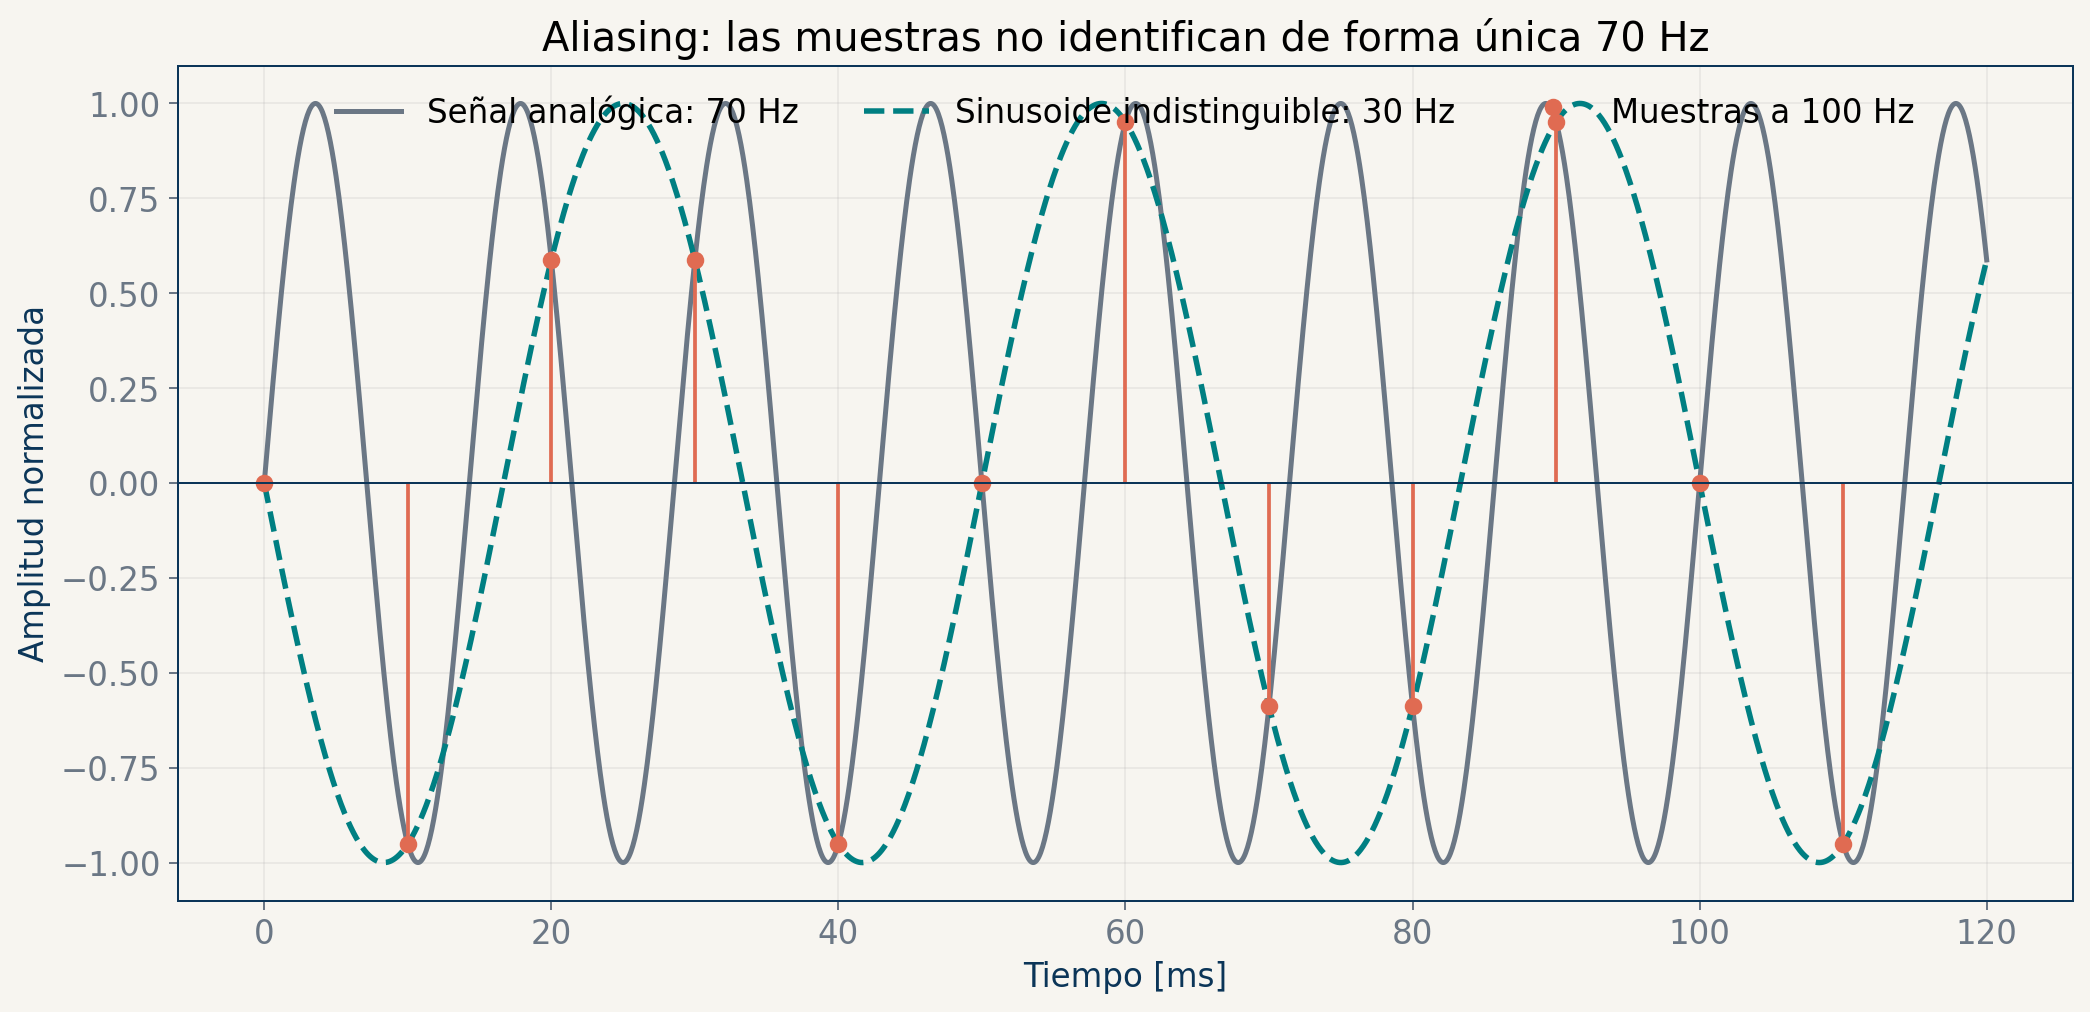
\includegraphics[width=0.91\linewidth,height=\textheight,keepaspectratio]{assets/aliasing.png}

\begin{tcolorbox}[enhanced jigsaw, bottomrule=.15mm, opacitybacktitle=0.6, rightrule=.15mm, opacityback=0, left=2mm, leftrule=.75mm, title={Lectura de la figura}, coltitle=black, colbacktitle=quarto-callout-warning-color!10!white, toprule=.15mm, colframe=quarto-callout-warning-color-frame, bottomtitle=1mm, toptitle=1mm, breakable, titlerule=0mm, arc=.35mm, colback=white]

Con \(f_s=100\) Hz, 70 Hz y 30 Hz generan secuencias indistinguibles
salvo por fase/signo. Aumentar bits no resuelve esta ambigüedad
temporal.

\end{tcolorbox}
\end{frame}

\begin{frame}{El filtro antialias debe ser analógico}
\phantomsection\label{el-filtro-antialias-debe-ser-analuxf3gico}
Antes del ADC se requiere un pasa-bajas que atenúe contenido por encima
de la banda admisible.

\begin{longtable}[]{@{}ll@{}}
\toprule\noalign{}
Parámetro & Significado \\
\midrule\noalign{}
\endhead
\(f_p\) & Fin de banda que debe conservarse \\
\(f_{st}\) & Inicio de banda que debe rechazarse \\
\(A_p\) & Pérdida máxima admisible en banda pasante \\
\(A_s\) & Atenuación mínima requerida en rechazo \\
\(f_s/2\) & Límite de Nyquist \\
\bottomrule\noalign{}
\end{longtable}

\begin{tcolorbox}[enhanced jigsaw, bottomrule=.15mm, opacitybacktitle=0.6, rightrule=.15mm, opacityback=0, left=2mm, leftrule=.75mm, title={Orden causal de las operaciones}, coltitle=black, colbacktitle=quarto-callout-important-color!10!white, toprule=.15mm, colframe=quarto-callout-important-color-frame, bottomtitle=1mm, toptitle=1mm, breakable, titlerule=0mm, arc=.35mm, colback=white]

Una componente que ya se plegó dentro de la banda después de muestrear
no puede identificarse como alias mediante un filtro digital ordinario.

\end{tcolorbox}
\end{frame}

\begin{frame}{Elegir \(f_s\): Nyquist es el piso teórico}
\phantomsection\label{elegir-f_s-nyquist-es-el-piso-teuxf3rico}
Ejemplo: si una medición EMG debe conservar hasta 450 Hz:

\begin{itemize}
\tightlist
\item
  \(f_s=900\) Hz deja transición nula: no es realizable.
\item
  \(f_s=1000\) Hz deja solo 50 Hz entre 450 Hz y Nyquist.
\item
  \(f_s=2000\) Hz deja 550 Hz para transición y simplifica el antialias.
\end{itemize}

La elección también depende de:

\begin{itemize}
\tightlist
\item
  memoria y transmisión;
\item
  sincronización entre canales;
\item
  latencia y carga de cómputo;
\item
  ancho de banda real del sensor.
\end{itemize}

\begin{tcolorbox}[enhanced jigsaw, bottomrule=.15mm, opacitybacktitle=0.6, rightrule=.15mm, opacityback=0, left=2mm, leftrule=.75mm, title={Criterio}, coltitle=black, colbacktitle=quarto-callout-note-color!10!white, toprule=.15mm, colframe=quarto-callout-note-color-frame, bottomtitle=1mm, toptitle=1mm, breakable, titlerule=0mm, arc=.35mm, colback=white]

Justifique \(f_s\) con banda útil, transición del filtro analógico y
recursos del sistema.

\end{tcolorbox}
\end{frame}

\begin{frame}{Cuantizar es discretizar la amplitud}
\phantomsection\label{cuantizar-es-discretizar-la-amplitud}
Para un cuantizador uniforme de \(N\) bits y rango \(V_{max}-V_{min}\):

\[
L=2^N,\qquad \Delta=\frac{V_{max}-V_{min}}{2^N}.
\]

Si no hay sobrecarga y se redondea al nivel más cercano:

\[
-\frac{\Delta}{2}\le e_q < \frac{\Delta}{2}.
\]

\begin{tcolorbox}[enhanced jigsaw, bottomrule=.15mm, opacitybacktitle=0.6, rightrule=.15mm, opacityback=0, left=2mm, leftrule=.75mm, title={Distinción}, coltitle=black, colbacktitle=quarto-callout-important-color!10!white, toprule=.15mm, colframe=quarto-callout-important-color-frame, bottomtitle=1mm, toptitle=1mm, breakable, titlerule=0mm, arc=.35mm, colback=white]

La frecuencia de muestreo controla resolución temporal; los bits
controlan resolución de amplitud. Son ejes diferentes.

\end{tcolorbox}
\end{frame}

\begin{frame}[shrink]{Más bits reducen el escalón, no evitan clipping}
\phantomsection\label{muxe1s-bits-reducen-el-escaluxf3n-no-evitan-clipping}
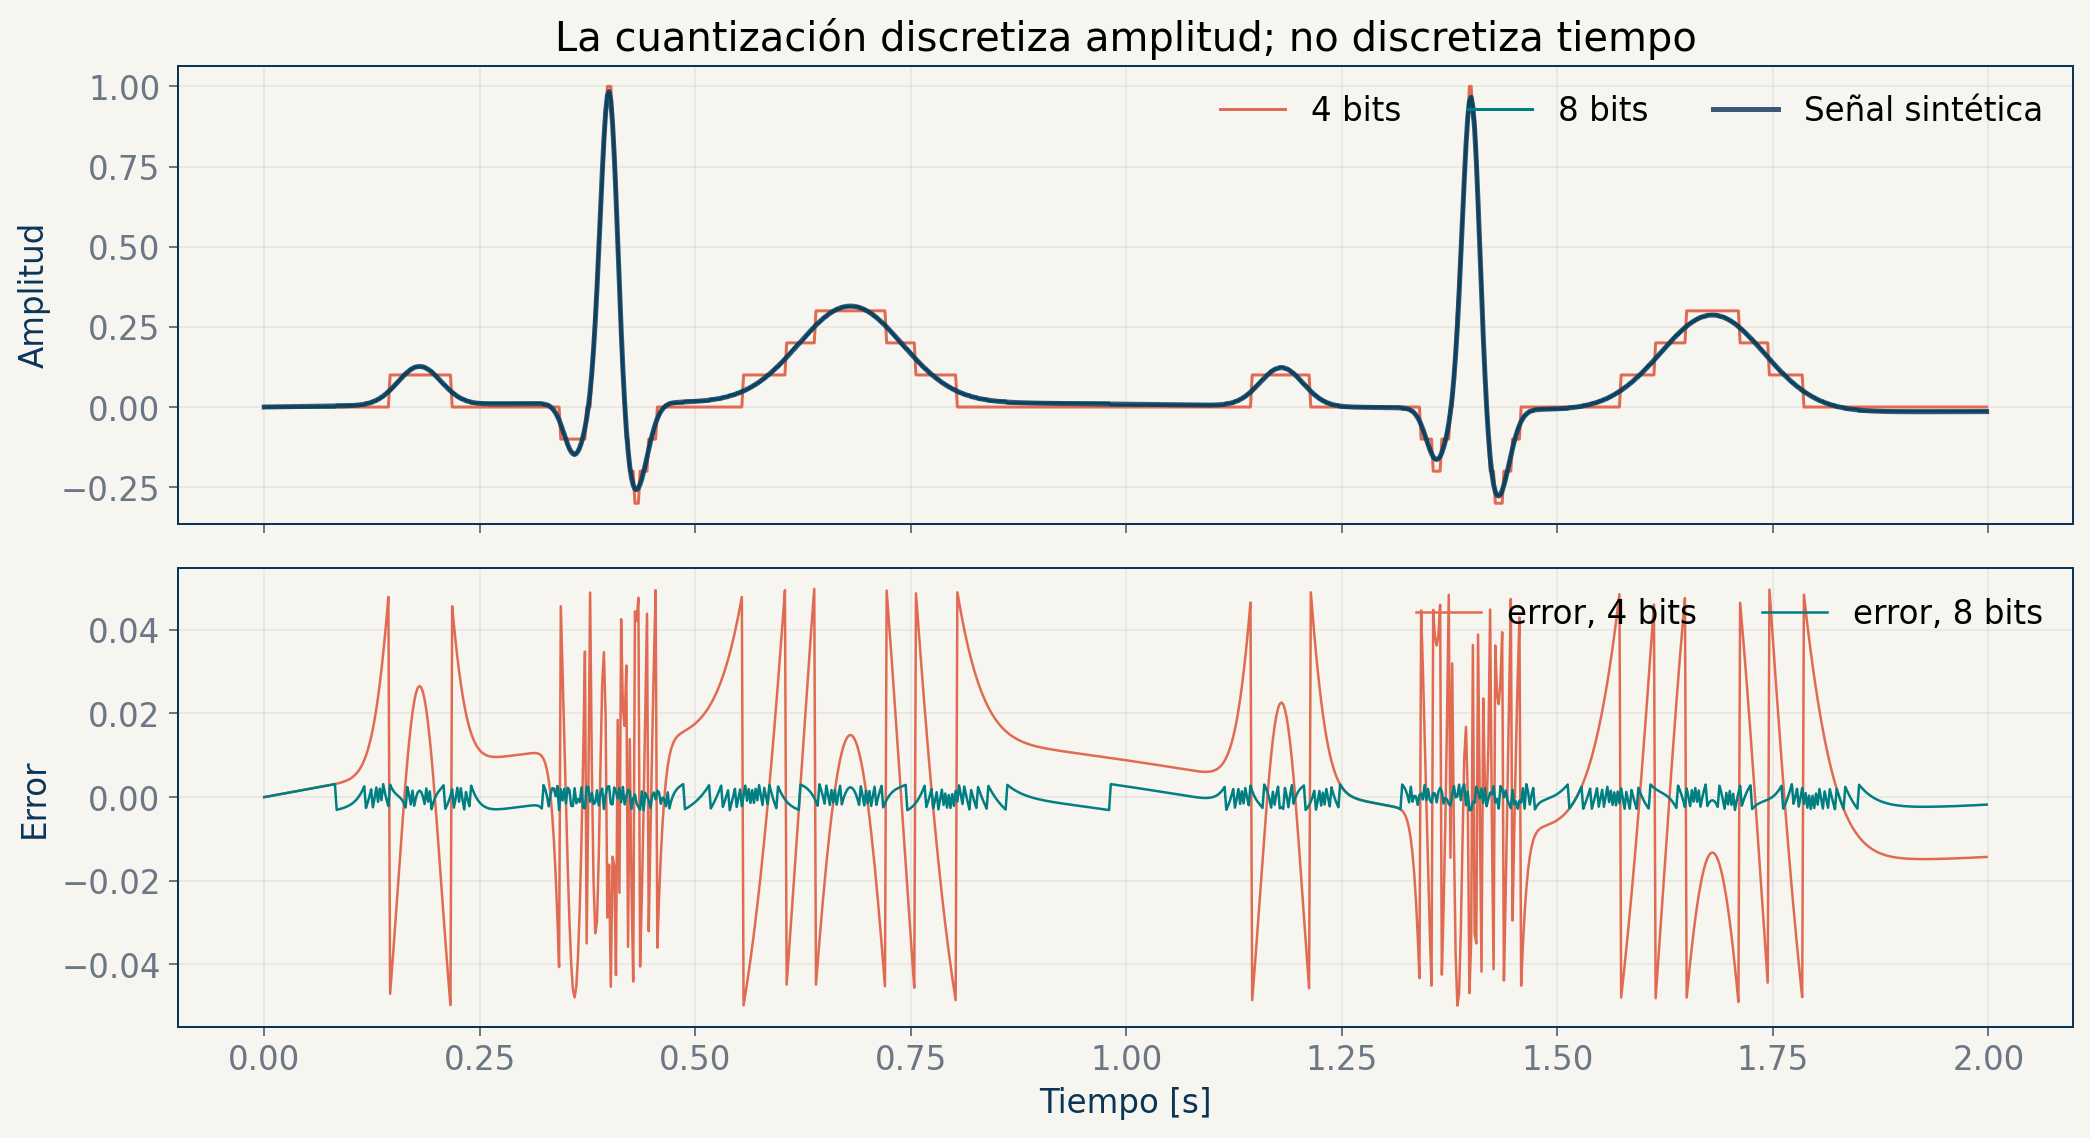
\includegraphics[width=0.9\linewidth,height=\textheight,keepaspectratio]{assets/quantization.png}

El ejemplo usa una señal tipo ECG \textbf{sintética}. No representa un
registro clínico.

\begin{tcolorbox}[enhanced jigsaw, bottomrule=.15mm, opacitybacktitle=0.6, rightrule=.15mm, opacityback=0, left=2mm, leftrule=.75mm, title={Observación}, coltitle=black, colbacktitle=quarto-callout-warning-color!10!white, toprule=.15mm, colframe=quarto-callout-warning-color-frame, bottomtitle=1mm, toptitle=1mm, breakable, titlerule=0mm, arc=.35mm, colback=white]

Si la señal excede el rango, todos los bits adicionales codifican el
mismo límite saturado. Primero se asegura el rango; después se discute
resolución.

\end{tcolorbox}
\end{frame}

\begin{frame}{El modelo de ruido de cuantización tiene supuestos}
\phantomsection\label{el-modelo-de-ruido-de-cuantizaciuxf3n-tiene-supuestos}
Bajo condiciones de señal suficientemente variable y sin sobrecarga:

\[
\sigma_q^2\approx \frac{\Delta^2}{12}.
\]

La regla aproximada para una sinusoide a escala completa es

\[
\mathrm{SQNR}_{\mathrm{dB}}\approx 6.02N+1.76.
\]

No debe extrapolarse sin revisión a señales:

\begin{itemize}
\tightlist
\item
  de muy baja amplitud respecto a \(\Delta\);
\item
  periódicas y sincronizadas con el cuantizador;
\item
  recortadas o con offset;
\item
  dominadas por ruido analógico.
\end{itemize}
\end{frame}

\begin{frame}{ENOB resume imperfecciones reales del convertidor}
\phantomsection\label{enob-resume-imperfecciones-reales-del-convertidor}
El número efectivo de bits puede estimarse desde SINAD:

\[
\mathrm{ENOB}=\frac{\mathrm{SINAD}_{\mathrm{dB}}-1.76}{6.02}.
\]

ENOB incorpora, de forma agregada, ruido y distorsión del sistema de
conversión.

\begin{tcolorbox}[enhanced jigsaw, bottomrule=.15mm, opacitybacktitle=0.6, rightrule=.15mm, opacityback=0, left=2mm, leftrule=.75mm, title={No confundir}, coltitle=black, colbacktitle=quarto-callout-note-color!10!white, toprule=.15mm, colframe=quarto-callout-note-color-frame, bottomtitle=1mm, toptitle=1mm, breakable, titlerule=0mm, arc=.35mm, colback=white]

Un ADC de 16 bits nominales no garantiza 16 bits efectivos en la banda,
ganancia y frecuencia de operación usadas.

\end{tcolorbox}
\end{frame}

\begin{frame}[fragile]{Código mínimo para cuantización uniforme}
\phantomsection\label{cuxf3digo-muxednimo-para-cuantizaciuxf3n-uniforme}
\begin{Shaded}
\begin{Highlighting}[]
\ImportTok{import}\NormalTok{ numpy }\ImportTok{as}\NormalTok{ np}

\KeywordTok{def}\NormalTok{ quantize(x, bits, vmin, vmax):}
\NormalTok{    levels }\OperatorTok{=} \DecValTok{2}\OperatorTok{**}\NormalTok{bits}
\NormalTok{    delta }\OperatorTok{=}\NormalTok{ (vmax }\OperatorTok{{-}}\NormalTok{ vmin) }\OperatorTok{/}\NormalTok{ levels}
\NormalTok{    x\_clip }\OperatorTok{=}\NormalTok{ np.clip(x, vmin, vmax }\OperatorTok{{-}}\NormalTok{ delta)}
\NormalTok{    codes }\OperatorTok{=}\NormalTok{ np.}\BuiltInTok{round}\NormalTok{((x\_clip }\OperatorTok{{-}}\NormalTok{ vmin) }\OperatorTok{/}\NormalTok{ delta)}
    \ControlFlowTok{return}\NormalTok{ vmin }\OperatorTok{+}\NormalTok{ codes }\OperatorTok{*}\NormalTok{ delta, delta}
\end{Highlighting}
\end{Shaded}

\begin{tcolorbox}[enhanced jigsaw, bottomrule=.15mm, opacitybacktitle=0.6, rightrule=.15mm, opacityback=0, left=2mm, leftrule=.75mm, title={Verificación computacional}, coltitle=black, colbacktitle=quarto-callout-tip-color!10!white, toprule=.15mm, colframe=quarto-callout-tip-color-frame, bottomtitle=1mm, toptitle=1mm, breakable, titlerule=0mm, arc=.35mm, colback=white]

Compruebe por separado porcentaje de muestras recortadas, \(\Delta\),
distribución del error y amplitud de los eventos de interés.

\end{tcolorbox}
\end{frame}

\begin{frame}{Checklist de adquisición biomédica}
\phantomsection\label{checklist-de-adquisiciuxf3n-biomuxe9dica}
\begin{itemize}
\tightlist
\item[$\square$]
  Variable fisiológica, unidades y montaje documentados.
\item[$\square$]
  Rango y ganancia definidos con margen.
\item[$\square$]
  Banda útil y antialias coherentes con \(f_s\).
\item[$\square$]
  Resolución de amplitud coherente con el evento mínimo.
\item[$\square$]
  Sincronización, reloj y pérdida de paquetes evaluados.
\item[$\square$]
  Saturación y desconexiones detectables.
\item[$\square$]
  Metadatos suficientes para reproducir el protocolo.
\end{itemize}

\begin{tcolorbox}[enhanced jigsaw, bottomrule=.15mm, opacitybacktitle=0.6, rightrule=.15mm, opacityback=0, left=2mm, leftrule=.75mm, title={Principio rector}, coltitle=black, colbacktitle=quarto-callout-important-color!10!white, toprule=.15mm, colframe=quarto-callout-important-color-frame, bottomtitle=1mm, toptitle=1mm, breakable, titlerule=0mm, arc=.35mm, colback=white]

La calidad del análisis digital está acotada por la información que la
adquisición logró preservar.

\end{tcolorbox}

Apoyo: Esakkirajan, Veerakumar y Subudhi (2024), cap. 2,
doi:10.1007/978-981-99-6752-0.
\end{frame}

\begin{frame}{Cierre de la semana 6}
\phantomsection\label{cierre-de-la-semana-6}
\begin{tcolorbox}[enhanced jigsaw, bottomrule=.15mm, opacitybacktitle=0.6, rightrule=.15mm, opacityback=0, left=2mm, leftrule=.75mm, title={Síntesis}, coltitle=black, colbacktitle=quarto-callout-important-color!10!white, toprule=.15mm, colframe=quarto-callout-important-color-frame, bottomtitle=1mm, toptitle=1mm, breakable, titlerule=0mm, arc=.35mm, colback=white]

Muestreo y cuantización limitan dimensiones distintas. El filtro
antialias debe actuar antes del ADC, y ningún aumento de bits recupera
información plegada o recortada.

\end{tcolorbox}
\end{frame}

\section{Semana 7 · Sesión 1}\label{semana-7-sesiuxf3n-1}

\begin{frame}{Modelar una transformación exige declarar sus propiedades}
\phantomsection\label{modelar-una-transformaciuxf3n-exige-declarar-sus-propiedades}
\textbf{Resultados de aprendizaje}

\begin{itemize}
\tightlist
\item
  Expresar un sistema como operador entrada-salida.
\item
  Evaluar linealidad, invariancia temporal, causalidad, memoria y
  estabilidad.
\item
  Relacionar propiedades matemáticas con riesgos de interpretación
  biomédica.
\end{itemize}

\textbf{Pregunta de entrada:} ¿todo algoritmo de procesamiento es un
filtro LTI?
\end{frame}

\begin{frame}{Un sistema es una regla que transforma señales}
\phantomsection\label{un-sistema-es-una-regla-que-transforma-seuxf1ales}
\[
y=\mathcal{T}\{x\}.
\]

Representaciones habituales:

\begin{itemize}
\tightlist
\item
  ecuación diferencial o en diferencias;
\item
  respuesta al impulso y convolución;
\item
  función de transferencia;
\item
  ecuaciones de estado;
\item
  algoritmo computacional.
\end{itemize}

\begin{tcolorbox}[enhanced jigsaw, bottomrule=.15mm, opacitybacktitle=0.6, rightrule=.15mm, opacityback=0, left=2mm, leftrule=.75mm, title={Concepto principal}, coltitle=black, colbacktitle=quarto-callout-important-color!10!white, toprule=.15mm, colframe=quarto-callout-important-color-frame, bottomtitle=1mm, toptitle=1mm, breakable, titlerule=0mm, arc=.35mm, colback=white]

Dos implementaciones son equivalentes solo si producen la misma relación
entrada-salida bajo los mismos supuestos y condiciones iniciales.

\end{tcolorbox}
\end{frame}

\begin{frame}{Memoria: ¿la salida usa otras muestras?}
\phantomsection\label{memoria-la-salida-usa-otras-muestras}
Sin memoria:

\[
y[n]=x^2[n].
\]

Con memoria:

\[
y[n]=\frac{x[n]+x[n-1]+x[n-2]}{3}.
\]

En bioseñales, una estimación de RMS móvil, una derivada o un filtro
digital tienen memoria.

\begin{tcolorbox}[enhanced jigsaw, bottomrule=.15mm, opacitybacktitle=0.6, rightrule=.15mm, opacityback=0, left=2mm, leftrule=.75mm, title={Prueba rápida}, coltitle=black, colbacktitle=quarto-callout-note-color!10!white, toprule=.15mm, colframe=quarto-callout-note-color-frame, bottomtitle=1mm, toptitle=1mm, breakable, titlerule=0mm, arc=.35mm, colback=white]

Si cambiar \(x[k]\) para \(k\neq n\) puede modificar \(y[n]\), el
sistema tiene memoria.

\end{tcolorbox}
\end{frame}

\begin{frame}[fragile]{Causalidad: presente y pasado, nunca futuro}
\phantomsection\label{causalidad-presente-y-pasado-nunca-futuro}
Un sistema discreto es causal si \(y[n_0]\) depende solo de \(x[n]\) con
\(n\le n_0\).

\begin{longtable}[]{@{}lrl@{}}
\toprule\noalign{}
Operación & ¿Causal? & Uso típico \\
\midrule\noalign{}
\endhead
\(y[n]=x[n]-x[n-1]\) & Sí & Tiempo real \\
\(y[n]=x[n+1]\) & No & Solo con datos futuros disponibles \\
Promedio centrado & No & Análisis fuera de línea \\
\texttt{sosfiltfilt} & No & Corrección de fase fuera de línea \\
\bottomrule\noalign{}
\end{longtable}

\begin{tcolorbox}[enhanced jigsaw, bottomrule=.15mm, opacitybacktitle=0.6, rightrule=.15mm, opacityback=0, left=2mm, leftrule=.75mm, title={Implicación}, coltitle=black, colbacktitle=quarto-callout-warning-color!10!white, toprule=.15mm, colframe=quarto-callout-warning-color-frame, bottomtitle=1mm, toptitle=1mm, breakable, titlerule=0mm, arc=.35mm, colback=white]

Un método no causal puede ser válido para análisis retrospectivo, pero
no para monitoreo en tiempo real.

\end{tcolorbox}
\end{frame}

\begin{frame}{Linealidad exige aditividad y homogeneidad}
\phantomsection\label{linealidad-exige-aditividad-y-homogeneidad}
\[
\mathcal{T}\{a x_1+b x_2\}=a\mathcal{T}\{x_1\}+b\mathcal{T}\{x_2\}.
\]

\begin{itemize}
\tightlist
\item
  \(y[n]=3x[n]\): lineal.
\item
  \(y[n]=x[n]+2\): no lineal por el offset.
\item
  \(y[n]=|x[n]|\): no lineal.
\item
  Saturación: no lineal.
\end{itemize}

\begin{tcolorbox}[enhanced jigsaw, bottomrule=.15mm, opacitybacktitle=0.6, rightrule=.15mm, opacityback=0, left=2mm, leftrule=.75mm, title={Consecuencia}, coltitle=black, colbacktitle=quarto-callout-important-color!10!white, toprule=.15mm, colframe=quarto-callout-important-color-frame, bottomtitle=1mm, toptitle=1mm, breakable, titlerule=0mm, arc=.35mm, colback=white]

Rectificar EMG cambia su contenido espectral porque la rectificación no
es una operación lineal.

\end{tcolorbox}
\end{frame}

\begin{frame}{Invariancia temporal: la regla no cambia con el reloj}
\phantomsection\label{invariancia-temporal-la-regla-no-cambia-con-el-reloj}
Si \(y[n]=\mathcal{T}\{x[n]\}\), un sistema invariante cumple

\[
\mathcal{T}\{x[n-n_0]\}=y[n-n_0].
\]

Ejemplos:

\begin{itemize}
\tightlist
\item
  Coeficientes fijos: potencialmente invariantes.
\item
  Ganancia dependiente de \(n\): variante en el tiempo.
\item
  Filtro adaptativo: deliberadamente variante.
\end{itemize}

\begin{tcolorbox}[enhanced jigsaw, bottomrule=.15mm, opacitybacktitle=0.6, rightrule=.15mm, opacityback=0, left=2mm, leftrule=.75mm, title={Contexto biomédico}, coltitle=black, colbacktitle=quarto-callout-note-color!10!white, toprule=.15mm, colframe=quarto-callout-note-color-frame, bottomtitle=1mm, toptitle=1mm, breakable, titlerule=0mm, arc=.35mm, colback=white]

La fisiología suele ser no estacionaria, aunque el filtro aplicado sea
LTI. No confunda propiedad del sistema con propiedad de la señal.

\end{tcolorbox}
\end{frame}

\begin{frame}{Estabilidad BIBO evita salidas no acotadas}
\phantomsection\label{estabilidad-bibo-evita-salidas-no-acotadas}
Un sistema es BIBO estable si toda entrada acotada produce salida
acotada.

Para un sistema LTI discreto:

\[
\sum_{n=-\infty}^{\infty}|h[n]|<\infty
\quad \Longrightarrow \quad \text{estabilidad BIBO}.
\]

\begin{tcolorbox}[enhanced jigsaw, bottomrule=.15mm, opacitybacktitle=0.6, rightrule=.15mm, opacityback=0, left=2mm, leftrule=.75mm, title={Importancia práctica}, coltitle=black, colbacktitle=quarto-callout-warning-color!10!white, toprule=.15mm, colframe=quarto-callout-warning-color-frame, bottomtitle=1mm, toptitle=1mm, breakable, titlerule=0mm, arc=.35mm, colback=white]

Un IIR con polos fuera del círculo unidad puede amplificar errores
numéricos y ruido hasta dominar la señal.

\end{tcolorbox}
\end{frame}

\begin{frame}{Las propiedades no vienen en paquete}
\phantomsection\label{las-propiedades-no-vienen-en-paquete}
\begin{longtable}[]{@{}lcccc@{}}
\toprule\noalign{}
Sistema & Lineal & Invariante & Causal & Estable \\
\midrule\noalign{}
\endhead
\(y[n]=x[n]+x[n-1]\) & Sí & Sí & Sí & Sí \\
\(y[n]=n\,x[n]\) & Sí & No & Sí & No necesariamente \\
\(y[n]=x[n+1]\) & Sí & Sí & No & Sí \\
\(y[n]=x^2[n]\) & No & Sí & Sí & Sí para entrada acotada \\
\bottomrule\noalign{}
\end{longtable}

\begin{tcolorbox}[enhanced jigsaw, bottomrule=.15mm, opacitybacktitle=0.6, rightrule=.15mm, opacityback=0, left=2mm, leftrule=.75mm, title={Método}, coltitle=black, colbacktitle=quarto-callout-tip-color!10!white, toprule=.15mm, colframe=quarto-callout-tip-color-frame, bottomtitle=1mm, toptitle=1mm, breakable, titlerule=0mm, arc=.35mm, colback=white]

Evalúe cada propiedad con su definición. No concluya causalidad o
estabilidad a partir de que el sistema sea lineal.

\end{tcolorbox}
\end{frame}

\begin{frame}{Verificación 7.1}
\phantomsection\label{verificaciuxf3n-7.1}
Considere \(y[n]=0.8y[n-1]+x[n]\).

\begin{enumerate}
\tightlist
\item
  ¿Tiene memoria?
\item
  ¿Es lineal e invariante si el coeficiente permanece fijo?
\item
  ¿Es causal?
\item
  ¿Qué propiedad del polo anticipa la estabilidad?
\end{enumerate}

\begin{tcolorbox}[enhanced jigsaw, bottomrule=.15mm, opacitybacktitle=0.6, rightrule=.15mm, opacityback=0, left=2mm, leftrule=.75mm, title={Respuesta esperada}, coltitle=black, colbacktitle=quarto-callout-note-color!10!white, toprule=.15mm, colframe=quarto-callout-note-color-frame, bottomtitle=1mm, toptitle=1mm, breakable, titlerule=0mm, arc=.35mm, colback=white]

Tiene memoria, es LTI y causal. Su polo está en \(0.8\), dentro del
círculo unidad; para la realización causal resulta BIBO estable.

\end{tcolorbox}
\end{frame}

\begin{frame}{Cierre de la sesión 13}
\phantomsection\label{cierre-de-la-sesiuxf3n-13}
\begin{tcolorbox}[enhanced jigsaw, bottomrule=.15mm, opacitybacktitle=0.6, rightrule=.15mm, opacityback=0, left=2mm, leftrule=.75mm, title={Síntesis}, coltitle=black, colbacktitle=quarto-callout-important-color!10!white, toprule=.15mm, colframe=quarto-callout-important-color-frame, bottomtitle=1mm, toptitle=1mm, breakable, titlerule=0mm, arc=.35mm, colback=white]

Las propiedades de memoria, causalidad, linealidad, invariancia y
estabilidad deben probarse por separado. Juntas determinan qué análisis
y qué implementación son válidos.

\end{tcolorbox}
\end{frame}

\section{Semana 7 · Sesión 2}\label{semana-7-sesiuxf3n-2}

\begin{frame}{La respuesta al impulso determina un sistema LTI}
\phantomsection\label{la-respuesta-al-impulso-determina-un-sistema-lti}
\textbf{Resultados de aprendizaje}

\begin{itemize}
\tightlist
\item
  Derivar la convolución desde la descomposición en impulsos.
\item
  Calcular convolución discreta y reconocer soporte y retardo.
\item
  Interpretar suavizado y respuesta transitoria.
\end{itemize}

\textbf{Pregunta de entrada:} ¿por qué conocer \(h[n]\) permite predecir
cualquier salida?
\end{frame}

\begin{frame}[shrink]{Toda secuencia puede escribirse con impulsos
desplazados}
\phantomsection\label{toda-secuencia-puede-escribirse-con-impulsos-desplazados}
\[
x[n]=\sum_{k=-\infty}^{\infty}x[k]\,\delta[n-k].
\]

Si el sistema es lineal e invariante:

\[
\mathcal{T}\{\delta[n-k]\}=h[n-k].
\]

Por superposición:

\[
y[n]=\sum_{k=-\infty}^{\infty}x[k]h[n-k]=(x*h)[n].
\]

\begin{tcolorbox}[enhanced jigsaw, bottomrule=.15mm, opacitybacktitle=0.6, rightrule=.15mm, opacityback=0, left=2mm, leftrule=.75mm, title={Concepto principal}, coltitle=black, colbacktitle=quarto-callout-important-color!10!white, toprule=.15mm, colframe=quarto-callout-important-color-frame, bottomtitle=1mm, toptitle=1mm, breakable, titlerule=0mm, arc=.35mm, colback=white]

La convolución no es una receta aislada: es la consecuencia de
linealidad e invariancia temporal.

\end{tcolorbox}
\end{frame}

\begin{frame}{Convolución: invertir, desplazar, multiplicar y sumar}
\phantomsection\label{convoluciuxf3n-invertir-desplazar-multiplicar-y-sumar}
\[
y[n]=\sum_k x[k]h[n-k].
\]

Para un \(n\) fijo:

\begin{enumerate}
\tightlist
\item
  Invierta \(h[k]\to h[-k]\).
\item
  Desplace \(h[-k]\to h[n-k]\).
\item
  Multiplique punto a punto por \(x[k]\).
\item
  Sume sobre \(k\).
\end{enumerate}

\begin{tcolorbox}[enhanced jigsaw, bottomrule=.15mm, opacitybacktitle=0.6, rightrule=.15mm, opacityback=0, left=2mm, leftrule=.75mm, title={Error frecuente}, coltitle=black, colbacktitle=quarto-callout-warning-color!10!white, toprule=.15mm, colframe=quarto-callout-warning-color-frame, bottomtitle=1mm, toptitle=1mm, breakable, titlerule=0mm, arc=.35mm, colback=white]

Mover \(h[k-n]\) en lugar de \(h[n-k]\) cambia el resultado. Verifique
siempre el índice dentro de la suma.

\end{tcolorbox}
\end{frame}

\begin{frame}[shrink]{Un promedio móvil ensancha bordes y reduce
variación rápida}
\phantomsection\label{un-promedio-muxf3vil-ensancha-bordes-y-reduce-variaciuxf3n-ruxe1pida}
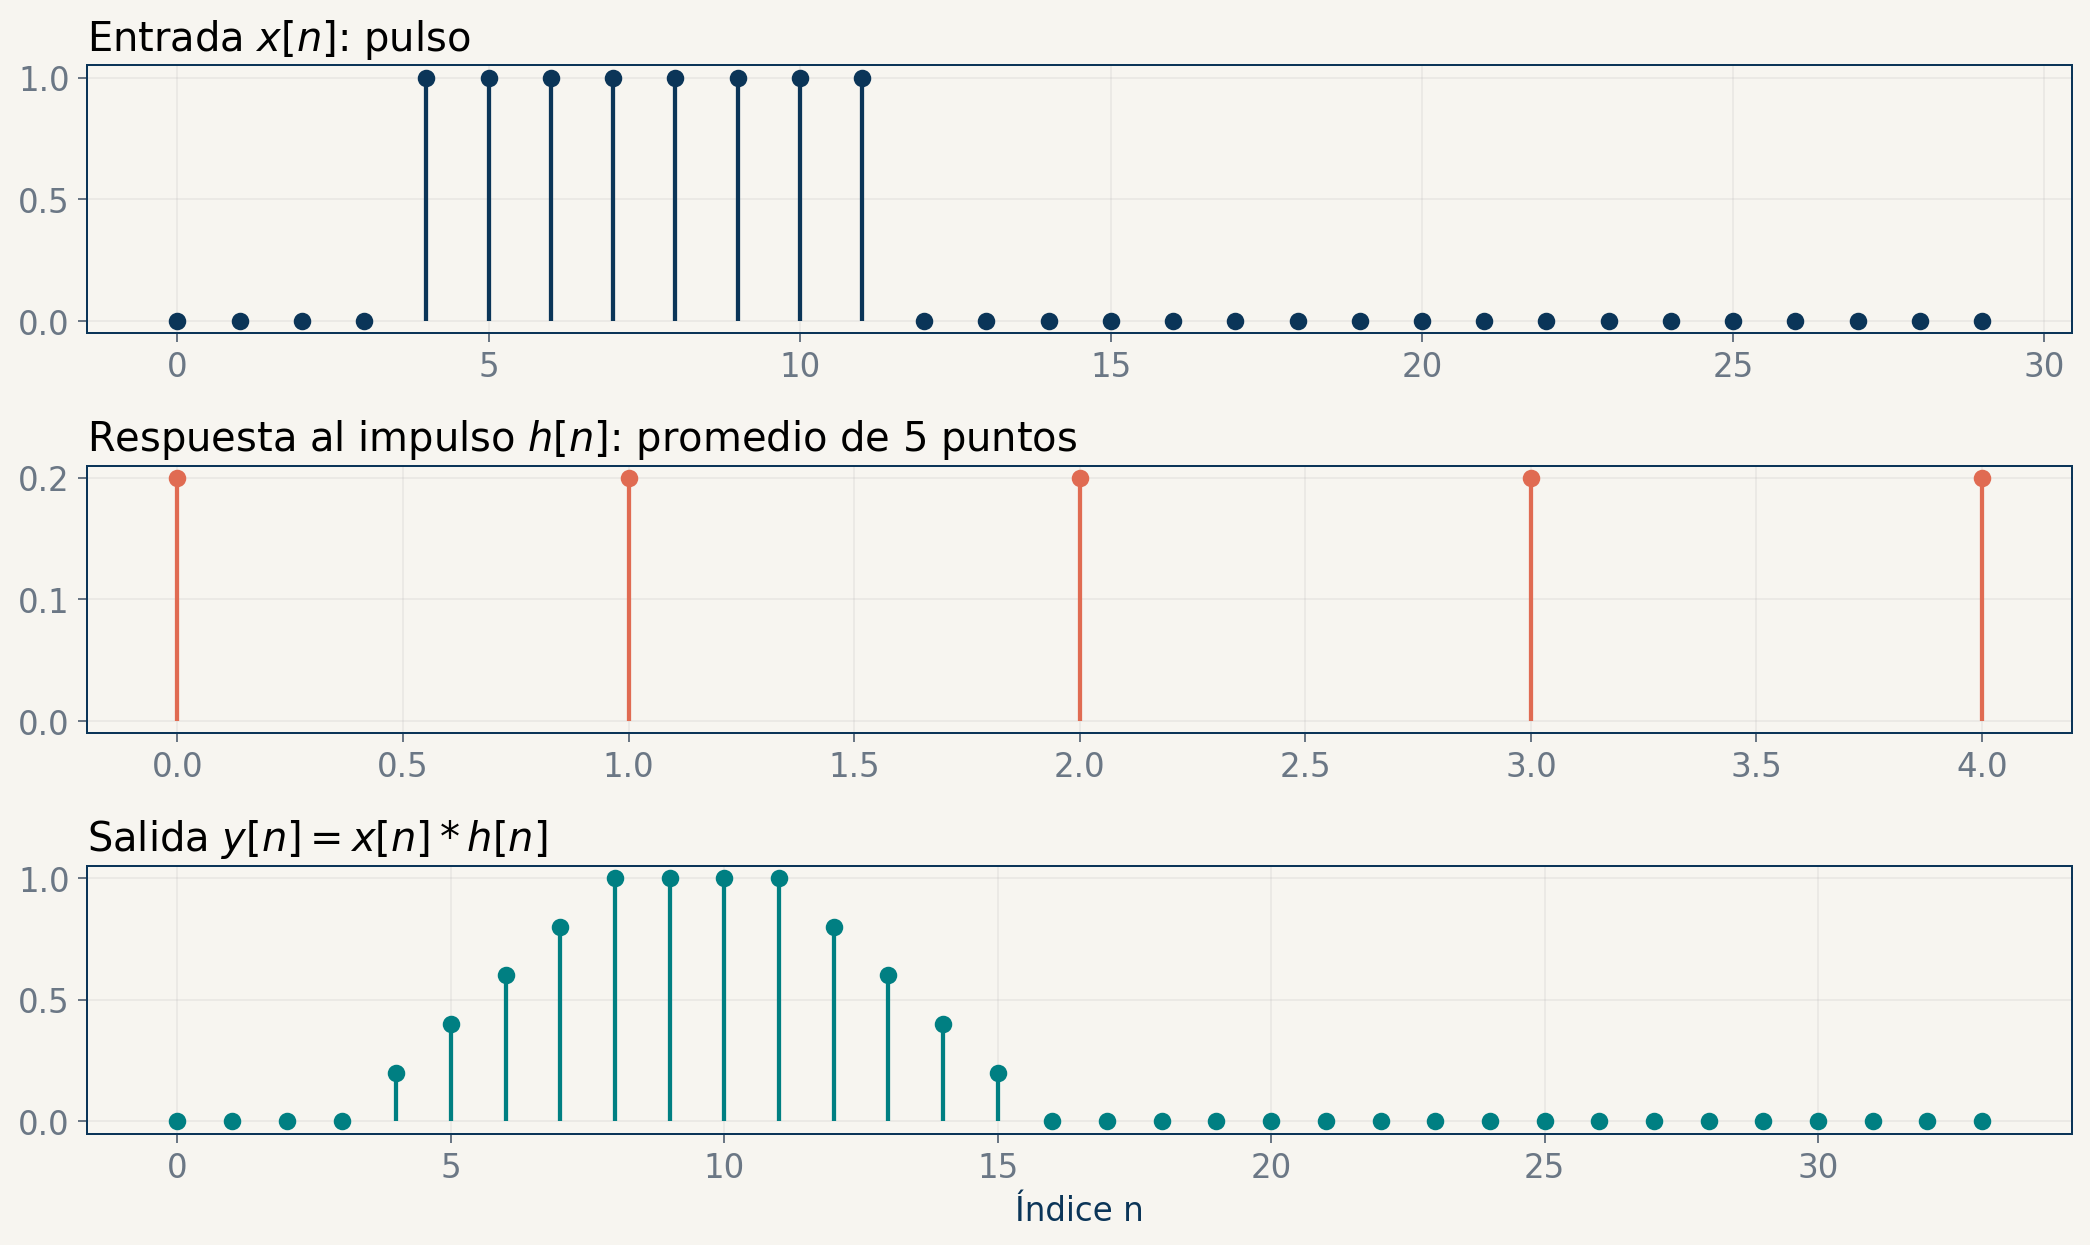
\includegraphics[width=0.86\linewidth,height=\textheight,keepaspectratio]{assets/convolution.png}

\begin{tcolorbox}[enhanced jigsaw, bottomrule=.15mm, opacitybacktitle=0.6, rightrule=.15mm, opacityback=0, left=2mm, leftrule=.75mm, title={Lectura}, coltitle=black, colbacktitle=quarto-callout-note-color!10!white, toprule=.15mm, colframe=quarto-callout-note-color-frame, bottomtitle=1mm, toptitle=1mm, breakable, titlerule=0mm, arc=.35mm, colback=white]

La rampa de entrada y salida aparece porque el promedio incluye
progresivamente más o menos muestras del pulso.

\end{tcolorbox}
\end{frame}

\begin{frame}{Longitud y soporte permiten anticipar la salida}
\phantomsection\label{longitud-y-soporte-permiten-anticipar-la-salida}
Si \(x[n]\) tiene longitud \(N\) y \(h[n]\) longitud \(M\):

\[
L_y=N+M-1.
\]

Si los soportes son \([n_{x0},n_{x1}]\) y \([n_{h0},n_{h1}]\):

\[
\mathrm{supp}(y)=[n_{x0}+n_{h0},\ n_{x1}+n_{h1}].
\]

\begin{tcolorbox}[enhanced jigsaw, bottomrule=.15mm, opacitybacktitle=0.6, rightrule=.15mm, opacityback=0, left=2mm, leftrule=.75mm, title={Control de errores}, coltitle=black, colbacktitle=quarto-callout-tip-color!10!white, toprule=.15mm, colframe=quarto-callout-tip-color-frame, bottomtitle=1mm, toptitle=1mm, breakable, titlerule=0mm, arc=.35mm, colback=white]

Antes de calcular valores, determine soporte, longitud y posibles
simetrías. Son pruebas independientes del código.

\end{tcolorbox}
\end{frame}

\begin{frame}{Convolución continua: el área de solapamiento cambia}
\phantomsection\label{convoluciuxf3n-continua-el-uxe1rea-de-solapamiento-cambia}
\[
y(t)=\int_{-\infty}^{\infty}x(\tau)h(t-\tau)\,d\tau.
\]

Para señales por tramos, los límites de integración dependen de \(t\).

\begin{itemize}
\tightlist
\item
  Sin solapamiento: \(y(t)=0\).
\item
  Solapamiento parcial: el intervalo crece o decrece.
\item
  Solapamiento total: puede aparecer una meseta.
\end{itemize}

\begin{tcolorbox}[enhanced jigsaw, bottomrule=.15mm, opacitybacktitle=0.6, rightrule=.15mm, opacityback=0, left=2mm, leftrule=.75mm, title={Interpretación geométrica}, coltitle=black, colbacktitle=quarto-callout-important-color!10!white, toprule=.15mm, colframe=quarto-callout-important-color-frame, bottomtitle=1mm, toptitle=1mm, breakable, titlerule=0mm, arc=.35mm, colback=white]

La integral suma productos solo donde \(x(\tau)\) y \(h(t-\tau)\) se
superponen.

\end{tcolorbox}
\end{frame}

\begin{frame}{El filtro promedio móvil es FIR y LTI}
\phantomsection\label{el-filtro-promedio-muxf3vil-es-fir-y-lti}
Para \(M\) muestras:

\[
h[n]=\begin{cases}
1/M, & 0\le n\le M-1,\\
0, & \text{otro caso}.
\end{cases}
\]

\[
y[n]=\frac{1}{M}\sum_{k=0}^{M-1}x[n-k].
\]

Efectos:

\begin{itemize}
\tightlist
\item
  suaviza cambios rápidos;
\item
  introduce retardo;
\item
  no separa selectivamente bandas cercanas;
\item
  conserva DC porque \(\sum h[n]=1\).
\end{itemize}
\end{frame}

\begin{frame}[fragile]{Código y prueba mínima de convolución}
\phantomsection\label{cuxf3digo-y-prueba-muxednima-de-convoluciuxf3n}
\begin{Shaded}
\begin{Highlighting}[]
\ImportTok{import}\NormalTok{ numpy }\ImportTok{as}\NormalTok{ np}

\NormalTok{x }\OperatorTok{=}\NormalTok{ np.array([}\DecValTok{0}\NormalTok{, }\DecValTok{1}\NormalTok{, }\DecValTok{1}\NormalTok{, }\DecValTok{1}\NormalTok{, }\DecValTok{0}\NormalTok{], dtype}\OperatorTok{=}\BuiltInTok{float}\NormalTok{)}
\NormalTok{h }\OperatorTok{=}\NormalTok{ np.ones(}\DecValTok{3}\NormalTok{) }\OperatorTok{/} \DecValTok{3}
\NormalTok{y }\OperatorTok{=}\NormalTok{ np.convolve(x, h, mode}\OperatorTok{=}\StringTok{"full"}\NormalTok{)}

\ControlFlowTok{assert} \BuiltInTok{len}\NormalTok{(y) }\OperatorTok{==} \BuiltInTok{len}\NormalTok{(x) }\OperatorTok{+} \BuiltInTok{len}\NormalTok{(h) }\OperatorTok{{-}} \DecValTok{1}
\ControlFlowTok{assert}\NormalTok{ np.isclose(h.}\BuiltInTok{sum}\NormalTok{(), }\FloatTok{1.0}\NormalTok{)}
\end{Highlighting}
\end{Shaded}

\begin{tcolorbox}[enhanced jigsaw, bottomrule=.15mm, opacitybacktitle=0.6, rightrule=.15mm, opacityback=0, left=2mm, leftrule=.75mm, title={Interpretación}, coltitle=black, colbacktitle=quarto-callout-note-color!10!white, toprule=.15mm, colframe=quarto-callout-note-color-frame, bottomtitle=1mm, toptitle=1mm, breakable, titlerule=0mm, arc=.35mm, colback=white]

La prueba de longitud detecta errores de modo o recorte; la suma
unitaria verifica ganancia DC, no toda la respuesta en frecuencia.

\end{tcolorbox}
\end{frame}

\begin{frame}[fragile]{Convolución, correlación y filtrado no son
intercambiables}
\phantomsection\label{convoluciuxf3n-correlaciuxf3n-y-filtrado-no-son-intercambiables}
\begin{longtable}[]{@{}
  >{\raggedright\arraybackslash}p{(\linewidth - 4\tabcolsep) * \real{0.3333}}
  >{\raggedright\arraybackslash}p{(\linewidth - 4\tabcolsep) * \real{0.3333}}
  >{\raggedright\arraybackslash}p{(\linewidth - 4\tabcolsep) * \real{0.3333}}@{}}
\toprule\noalign{}
\begin{minipage}[b]{\linewidth}\raggedright
Operación
\end{minipage} & \begin{minipage}[b]{\linewidth}\raggedright
Expresión
\end{minipage} & \begin{minipage}[b]{\linewidth}\raggedright
Pregunta que responde
\end{minipage} \\
\midrule\noalign{}
\endhead
Convolución & \(\sum x[k]h[n-k]\) & ¿Cuál es la salida del LTI? \\
Correlación & \(\sum x[k]y^*[k-n]\) & ¿Qué tan similares son a cierto
desfase? \\
Filtrado & Implementación de \(H\) & ¿Cómo modificar una señal según una
respuesta? \\
\bottomrule\noalign{}
\end{longtable}

\begin{tcolorbox}[enhanced jigsaw, bottomrule=.15mm, opacitybacktitle=0.6, rightrule=.15mm, opacityback=0, left=2mm, leftrule=.75mm, title={Convención}, coltitle=black, colbacktitle=quarto-callout-warning-color!10!white, toprule=.15mm, colframe=quarto-callout-warning-color-frame, bottomtitle=1mm, toptitle=1mm, breakable, titlerule=0mm, arc=.35mm, colback=white]

Las bibliotecas difieren en normalización, conjugación, retardos y modos
\texttt{full}, \texttt{same}, \texttt{valid}. Documente la definición
usada.

\end{tcolorbox}
\end{frame}

\begin{frame}[shrink]{Cierre de la semana 7}
\phantomsection\label{cierre-de-la-semana-7}
Puede modelar una operación como LTI cuando:

\begin{itemize}
\tightlist
\item
  cumple superposición;
\item
  su regla no cambia con el tiempo;
\item
  sus condiciones iniciales se tratan coherentemente.
\end{itemize}

Entonces \(h[n]\) permite estudiar:

\begin{itemize}
\tightlist
\item
  causalidad;
\item
  estabilidad;
\item
  respuesta transitoria;
\item
  respuesta en frecuencia.
\end{itemize}

\begin{tcolorbox}[enhanced jigsaw, bottomrule=.15mm, opacitybacktitle=0.6, rightrule=.15mm, opacityback=0, left=2mm, leftrule=.75mm, title={Puente a la semana 8}, coltitle=black, colbacktitle=quarto-callout-important-color!10!white, toprule=.15mm, colframe=quarto-callout-important-color-frame, bottomtitle=1mm, toptitle=1mm, breakable, titlerule=0mm, arc=.35mm, colback=white]

La convolución en tiempo se convierte en multiplicación en frecuencia.
Esa equivalencia hace operativo el análisis de Fourier.

\end{tcolorbox}
\end{frame}

\section{Semana 8 · Sesión 1}\label{semana-8-sesiuxf3n-1}

\begin{frame}{La transformada extiende Fourier a señales aperiódicas}
\phantomsection\label{la-transformada-extiende-fourier-a-seuxf1ales-aperiuxf3dicas}
\textbf{Resultados de aprendizaje}

\begin{itemize}
\tightlist
\item
  Pasar de la serie de Fourier a la transformada de señales aperiódicas.
\item
  Interpretar magnitud, fase y propiedades de la transformada.
\item
  Usar el teorema de convolución para analizar sistemas LTI.
\end{itemize}

\textbf{Pregunta de entrada:} si una señal no es periódica, ¿cómo puede
representarse mediante frecuencias?
\end{frame}

\begin{frame}{La transformada aparece al llevar el período al infinito}
\phantomsection\label{la-transformada-aparece-al-llevar-el-peruxedodo-al-infinito}
La serie compleja usa líneas separadas por \(\omega_0=2\pi/T_0\). Cuando
\(T_0\to\infty\), esa separación tiende a cero y la suma se convierte en
integral:

\[
X(\omega)=\int_{-\infty}^{\infty}x(t)e^{-j\omega t}\,dt.
\]

\[
x(t)=\frac{1}{2\pi}\int_{-\infty}^{\infty}X(\omega)e^{j\omega t}\,d\omega.
\]

\begin{tcolorbox}[enhanced jigsaw, bottomrule=.15mm, opacitybacktitle=0.6, rightrule=.15mm, opacityback=0, left=2mm, leftrule=.75mm, title={Continuidad con la semana 5}, coltitle=black, colbacktitle=quarto-callout-important-color!10!white, toprule=.15mm, colframe=quarto-callout-important-color-frame, bottomtitle=1mm, toptitle=1mm, breakable, titlerule=0mm, arc=.35mm, colback=white]

La serie describe espectros de líneas para señales periódicas; la
transformada describe un continuo de frecuencias para señales
aperiódicas.

\end{tcolorbox}
\end{frame}

\begin{frame}{Las exponenciales complejas son autofunciones LTI}
\phantomsection\label{las-exponenciales-complejas-son-autofunciones-lti}
Si \(x(t)=e^{j\omega t}\), entonces

\[
y(t)=h(t)*e^{j\omega t}
=H(j\omega)e^{j\omega t}.
\]

El sistema no cambia la frecuencia; multiplica por un número complejo:

\begin{itemize}
\tightlist
\item
  \(|H(j\omega)|\): escala amplitud;
\item
  \(\angle H(j\omega)\): desplaza fase.
\end{itemize}

\begin{tcolorbox}[enhanced jigsaw, bottomrule=.15mm, opacitybacktitle=0.6, rightrule=.15mm, opacityback=0, left=2mm, leftrule=.75mm, title={Por qué importa}, coltitle=black, colbacktitle=quarto-callout-note-color!10!white, toprule=.15mm, colframe=quarto-callout-note-color-frame, bottomtitle=1mm, toptitle=1mm, breakable, titlerule=0mm, arc=.35mm, colback=white]

Si una señal se descompone en frecuencias, basta conocer cómo el sistema
modifica cada componente.

\end{tcolorbox}
\end{frame}

\begin{frame}{Magnitud y fase responden preguntas diferentes}
\phantomsection\label{magnitud-y-fase-responden-preguntas-diferentes}
\[
X(\omega)=|X(\omega)|e^{j\phi(\omega)}.
\]

\begin{itemize}
\tightlist
\item
  La magnitud indica cuánto contribuye una frecuencia.
\item
  La fase indica cómo se alinean sus componentes temporales.
\item
  Dos señales pueden compartir magnitud y tener morfologías distintas
  por su fase.
\end{itemize}

\begin{tcolorbox}[enhanced jigsaw, bottomrule=.15mm, opacitybacktitle=0.6, rightrule=.15mm, opacityback=0, left=2mm, leftrule=.75mm, title={Error frecuente}, coltitle=black, colbacktitle=quarto-callout-warning-color!10!white, toprule=.15mm, colframe=quarto-callout-warning-color-frame, bottomtitle=1mm, toptitle=1mm, breakable, titlerule=0mm, arc=.35mm, colback=white]

Interpretar solo \(|X(\omega)|\) como si contuviera toda la estructura
temporal. La reconstrucción exige magnitud y fase.

\end{tcolorbox}
\end{frame}

\begin{frame}{La simetría conjugada caracteriza señales reales}
\phantomsection\label{la-simetruxeda-conjugada-caracteriza-seuxf1ales-reales}
Si \(x(t)\) es real:

\[
X(-\omega)=X^*(\omega).
\]

Por tanto:

\begin{itemize}
\tightlist
\item
  \(|X(-\omega)|=|X(\omega)|\);
\item
  \(\angle X(-\omega)=-\angle X(\omega)\), salvo ambigüedades de fase;
\item
  el espectro bilateral contiene redundancia para una señal real.
\end{itemize}

\begin{tcolorbox}[enhanced jigsaw, bottomrule=.15mm, opacitybacktitle=0.6, rightrule=.15mm, opacityback=0, left=2mm, leftrule=.75mm, title={Lectura correcta}, coltitle=black, colbacktitle=quarto-callout-note-color!10!white, toprule=.15mm, colframe=quarto-callout-note-color-frame, bottomtitle=1mm, toptitle=1mm, breakable, titlerule=0mm, arc=.35mm, colback=white]

La frecuencia negativa es parte de la representación compleja; no
corresponde a una oscilación fisiológica que transcurre hacia atrás.

\end{tcolorbox}
\end{frame}

\begin{frame}[shrink]{Las propiedades permiten predecir sin reintegrar}
\phantomsection\label{las-propiedades-permiten-predecir-sin-reintegrar}
\begin{longtable}[]{@{}ll@{}}
\toprule\noalign{}
Operación temporal & Efecto frecuencial \\
\midrule\noalign{}
\endhead
\(a x(t)+b y(t)\) & \(aX(\omega)+bY(\omega)\) \\
\(x(t-t_0)\) & \(e^{-j\omega t_0}X(\omega)\) \\
\(x(at)\) & \(\frac{1}{|a|}X(\omega/a)\) \\
\(\frac{d}{dt}x(t)\) & \(j\omega X(\omega)\) \\
\(x(t)e^{j\omega_0t}\) & \(X(\omega-\omega_0)\) \\
\bottomrule\noalign{}
\end{longtable}

\begin{tcolorbox}[enhanced jigsaw, bottomrule=.15mm, opacitybacktitle=0.6, rightrule=.15mm, opacityback=0, left=2mm, leftrule=.75mm, title={Método de estudio}, coltitle=black, colbacktitle=quarto-callout-tip-color!10!white, toprule=.15mm, colframe=quarto-callout-tip-color-frame, bottomtitle=1mm, toptitle=1mm, breakable, titlerule=0mm, arc=.35mm, colback=white]

Explique primero el efecto cualitativo. Luego use la propiedad y
verifique dimensiones, signo y factor de escala.

\end{tcolorbox}
\end{frame}

\begin{frame}{Convolución en tiempo es multiplicación en frecuencia}
\phantomsection\label{convoluciuxf3n-en-tiempo-es-multiplicaciuxf3n-en-frecuencia}
\[
y(t)=x(t)*h(t)
\quad\Longleftrightarrow\quad
Y(\omega)=X(\omega)H(\omega).
\]

El teorema permite:

\begin{itemize}
\tightlist
\item
  anticipar qué componentes se atenúan;
\item
  separar respuesta de la señal y respuesta del sistema;
\item
  diseñar \(H(\omega)\) desde una especificación;
\item
  validar resultados en dos dominios.
\end{itemize}

\begin{tcolorbox}[enhanced jigsaw, bottomrule=.15mm, opacitybacktitle=0.6, rightrule=.15mm, opacityback=0, left=2mm, leftrule=.75mm, title={Puente hacia filtrado}, coltitle=black, colbacktitle=quarto-callout-important-color!10!white, toprule=.15mm, colframe=quarto-callout-important-color-frame, bottomtitle=1mm, toptitle=1mm, breakable, titlerule=0mm, arc=.35mm, colback=white]

Un filtro LTI no «busca» eventos: pondera cada componente según su
respuesta compleja \(H(\omega)\).

\end{tcolorbox}
\end{frame}

\begin{frame}{Parseval conserva energía entre dominios}
\phantomsection\label{parseval-conserva-energuxeda-entre-dominios}
Con esta convención de transformada:

\[
\int_{-\infty}^{\infty}|x(t)|^2dt
=\frac{1}{2\pi}\int_{-\infty}^{\infty}|X(\omega)|^2d\omega.
\]

Aplicaciones:

\begin{itemize}
\tightlist
\item
  verificar transformadas y escalamiento;
\item
  comparar energía antes y después de filtrar;
\item
  cuantificar la fracción contenida en una banda.
\end{itemize}

\begin{tcolorbox}[enhanced jigsaw, bottomrule=.15mm, opacitybacktitle=0.6, rightrule=.15mm, opacityback=0, left=2mm, leftrule=.75mm, title={Convenciones}, coltitle=black, colbacktitle=quarto-callout-caution-color!10!white, toprule=.15mm, colframe=quarto-callout-caution-color-frame, bottomtitle=1mm, toptitle=1mm, breakable, titlerule=0mm, arc=.35mm, colback=white]

Los factores \(2\pi\) cambian según se use \(f\) en Hz o \(\omega\) en
rad/s. Declare el par de transformada.

\end{tcolorbox}
\end{frame}

\begin{frame}{Verificación 8.1}
\phantomsection\label{verificaciuxf3n-8.1}
Un sistema tiene \(|H(j\omega)|\approx 0\) por encima de \(40\) Hz y
fase no lineal en la banda pasante.

\begin{enumerate}
\tightlist
\item
  ¿Qué componentes atenúa?
\item
  ¿Puede conservar amplitud y deformar morfología?
\item
  ¿Qué propiedad explica esa deformación?
\end{enumerate}

\begin{tcolorbox}[enhanced jigsaw, bottomrule=.15mm, opacitybacktitle=0.6, rightrule=.15mm, opacityback=0, left=2mm, leftrule=.75mm, title={Criterio de respuesta}, coltitle=black, colbacktitle=quarto-callout-note-color!10!white, toprule=.15mm, colframe=quarto-callout-note-color-frame, bottomtitle=1mm, toptitle=1mm, breakable, titlerule=0mm, arc=.35mm, colback=white]

Atenúa principalmente contenido superior a 40 Hz. Sí puede alterar la
forma aunque conserve magnitud en la banda, porque distintos componentes
sufren desplazamientos de fase diferentes.

\end{tcolorbox}
\end{frame}

\begin{frame}{Cierre de la sesión 15}
\phantomsection\label{cierre-de-la-sesiuxf3n-15}
\begin{tcolorbox}[enhanced jigsaw, bottomrule=.15mm, opacitybacktitle=0.6, rightrule=.15mm, opacityback=0, left=2mm, leftrule=.75mm, title={Síntesis}, coltitle=black, colbacktitle=quarto-callout-important-color!10!white, toprule=.15mm, colframe=quarto-callout-important-color-frame, bottomtitle=1mm, toptitle=1mm, breakable, titlerule=0mm, arc=.35mm, colback=white]

\begin{itemize}
\tightlist
\item
  La transformada extiende la serie desde líneas armónicas hacia
  frecuencia continua.
\item
  Magnitud y fase son necesarias para describir la señal.
\item
  Las propiedades permiten anticipar efectos sin recalcular integrales.
\item
  El teorema de convolución conecta análisis de sistemas y filtrado.
\end{itemize}

\end{tcolorbox}
\end{frame}

\section{Semana 8 · Sesión 2}\label{semana-8-sesiuxf3n-2}

\begin{frame}{La DFT convierte un bloque finito en muestras espectrales}
\phantomsection\label{la-dft-convierte-un-bloque-finito-en-muestras-espectrales}
\textbf{Resultados de aprendizaje}

\begin{itemize}
\tightlist
\item
  Relacionar DTFS, DTFT y DFT sin confundir sus dominios.
\item
  Interpretar resolución frecuencial, fuga y ventanas.
\item
  Construir una lectura espectral que respete el contexto fisiológico.
\end{itemize}

\textbf{Pregunta de entrada:} ¿el pico mayor de la FFT es siempre la
frecuencia fisiológica dominante?
\end{frame}

\begin{frame}{Tres objetos distintos suelen llamarse ``Fourier''}
\phantomsection\label{tres-objetos-distintos-suelen-llamarse-fourier}
\begin{longtable}[]{@{}
  >{\raggedright\arraybackslash}p{(\linewidth - 6\tabcolsep) * \real{0.2500}}
  >{\raggedright\arraybackslash}p{(\linewidth - 6\tabcolsep) * \real{0.2500}}
  >{\raggedright\arraybackslash}p{(\linewidth - 6\tabcolsep) * \real{0.2500}}
  >{\raggedright\arraybackslash}p{(\linewidth - 6\tabcolsep) * \real{0.2500}}@{}}
\toprule\noalign{}
\begin{minipage}[b]{\linewidth}\raggedright
Representación
\end{minipage} & \begin{minipage}[b]{\linewidth}\raggedright
Señal de entrada
\end{minipage} & \begin{minipage}[b]{\linewidth}\raggedright
Variable frecuencial
\end{minipage} & \begin{minipage}[b]{\linewidth}\raggedright
Espectro
\end{minipage} \\
\midrule\noalign{}
\endhead
DTFS & Discreta y periódica & Índice \(k\) & Discreto y periódico \\
DTFT & Discreta aperiódica & \(\omega\) continua & Continuo y
periódico \\
DFT & Bloque finito de \(N\) muestras & \(k=0,\ldots,N-1\) & \(N\)
muestras frecuenciales \\
\bottomrule\noalign{}
\end{longtable}

\begin{tcolorbox}[enhanced jigsaw, bottomrule=.15mm, opacitybacktitle=0.6, rightrule=.15mm, opacityback=0, left=2mm, leftrule=.75mm, title={Concepto principal}, coltitle=black, colbacktitle=quarto-callout-important-color!10!white, toprule=.15mm, colframe=quarto-callout-important-color-frame, bottomtitle=1mm, toptitle=1mm, breakable, titlerule=0mm, arc=.35mm, colback=white]

La DFT analiza un registro finito como un período de una extensión
periódica. Sus resultados dependen de duración y ventana.

\end{tcolorbox}
\end{frame}

\begin{frame}[shrink]{La DFT y su inversa forman un par exacto}
\phantomsection\label{la-dft-y-su-inversa-forman-un-par-exacto}
\[
X[k]=\sum_{n=0}^{N-1}x[n]e^{-j2\pi kn/N},
\]

\[
x[n]=\frac{1}{N}\sum_{k=0}^{N-1}X[k]e^{j2\pi kn/N}.
\]

La frecuencia del bin \(k\) es

\[
f_k=\frac{k f_s}{N},\qquad \Delta f=\frac{f_s}{N}=\frac{1}{T}.
\]

\begin{tcolorbox}[enhanced jigsaw, bottomrule=.15mm, opacitybacktitle=0.6, rightrule=.15mm, opacityback=0, left=2mm, leftrule=.75mm, title={Interpretación}, coltitle=black, colbacktitle=quarto-callout-note-color!10!white, toprule=.15mm, colframe=quarto-callout-note-color-frame, bottomtitle=1mm, toptitle=1mm, breakable, titlerule=0mm, arc=.35mm, colback=white]

La resolución entre bins mejora principalmente al aumentar la duración
observada \(T\), no solo al aumentar \(f_s\).

\end{tcolorbox}
\end{frame}

\begin{frame}{La FFT acelera el cálculo; no cambia el significado}
\phantomsection\label{la-fft-acelera-el-cuxe1lculo-no-cambia-el-significado}
\begin{itemize}
\tightlist
\item
  DFT directa: orden aproximado \(O(N^2)\).
\item
  FFT: explota simetrías y reduce a \(O(N\log N)\).
\item
  La salida numérica representa la misma DFT.
\end{itemize}

\begin{tcolorbox}[enhanced jigsaw, bottomrule=.15mm, opacitybacktitle=0.6, rightrule=.15mm, opacityback=0, left=2mm, leftrule=.75mm, title={Error frecuente}, coltitle=black, colbacktitle=quarto-callout-warning-color!10!white, toprule=.15mm, colframe=quarto-callout-warning-color-frame, bottomtitle=1mm, toptitle=1mm, breakable, titlerule=0mm, arc=.35mm, colback=white]

Llamar ``FFT'' al espectro físico. FFT es el algoritmo; unidades,
normalización y eje frecuencial dependen de cómo se construya el
análisis.

\end{tcolorbox}
\end{frame}

\begin{frame}[shrink]{Fuga espectral: el segmento observado tiene
bordes}
\phantomsection\label{fuga-espectral-el-segmento-observado-tiene-bordes}
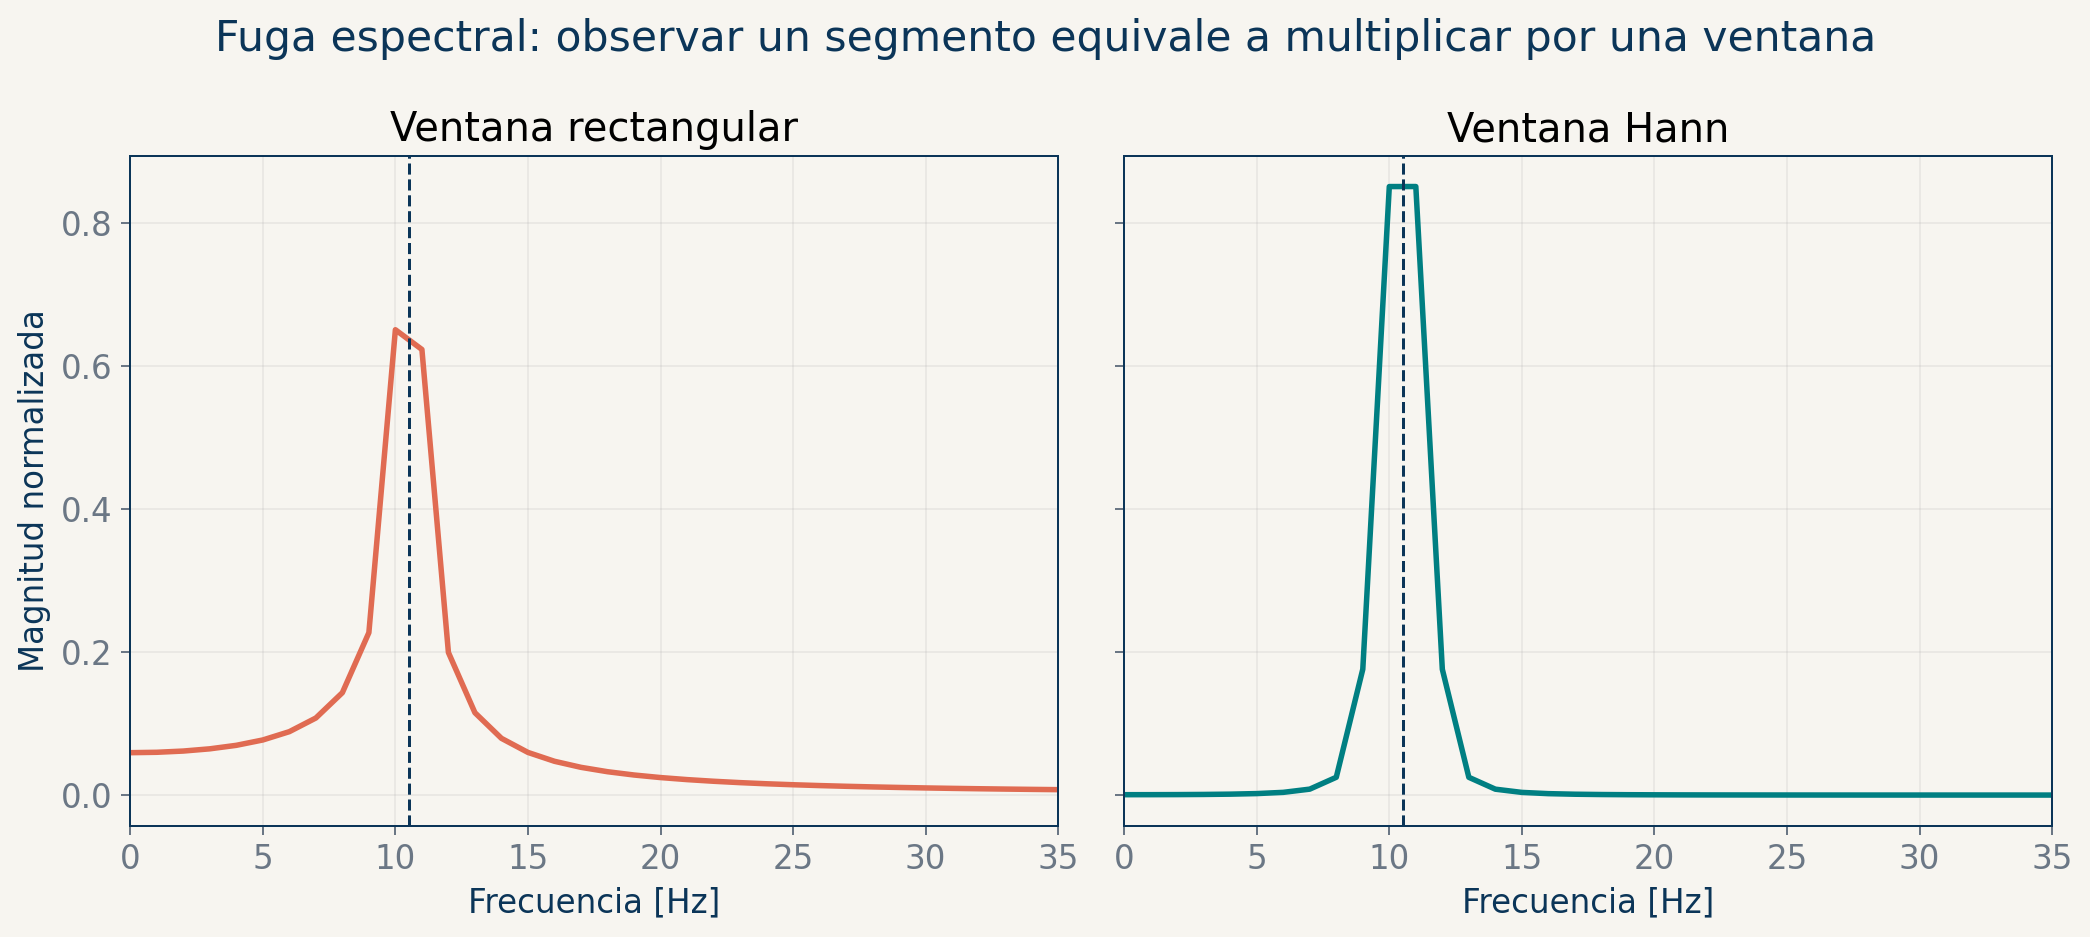
\includegraphics[width=0.88\linewidth,height=\textheight,keepaspectratio]{assets/spectral_leakage.png}

\begin{tcolorbox}[enhanced jigsaw, bottomrule=.15mm, opacitybacktitle=0.6, rightrule=.15mm, opacityback=0, left=2mm, leftrule=.75mm, title={Compromiso de las ventanas}, coltitle=black, colbacktitle=quarto-callout-important-color!10!white, toprule=.15mm, colframe=quarto-callout-important-color-frame, bottomtitle=1mm, toptitle=1mm, breakable, titlerule=0mm, arc=.35mm, colback=white]

Una ventana reduce lóbulos laterales a costa de ensanchar el lóbulo
principal y cambiar la ganancia. No existe una ventana óptima para todo
objetivo.

\end{tcolorbox}
\end{frame}

\begin{frame}{Zero padding interpola la gráfica, no la información}
\phantomsection\label{zero-padding-interpola-la-gruxe1fica-no-la-informaciuxf3n}
Agregar ceros aumenta el número de puntos evaluados en frecuencia:

\[
N_{FFT}>N.
\]

Pero la separación física de componentes cercanas sigue limitada por
duración, SNR y ventana.

\begin{tcolorbox}[enhanced jigsaw, bottomrule=.15mm, opacitybacktitle=0.6, rightrule=.15mm, opacityback=0, left=2mm, leftrule=.75mm, title={Diagnóstico}, coltitle=black, colbacktitle=quarto-callout-note-color!10!white, toprule=.15mm, colframe=quarto-callout-note-color-frame, bottomtitle=1mm, toptitle=1mm, breakable, titlerule=0mm, arc=.35mm, colback=white]

Una curva más suave no implica mayor capacidad para distinguir dos
frecuencias próximas.

\end{tcolorbox}
\end{frame}

\begin{frame}{Un espectro de amplitud exige normalización explícita}
\phantomsection\label{un-espectro-de-amplitud-exige-normalizaciuxf3n-expluxedcita}
Para una señal real y espectro unilateral:

\begin{enumerate}
\tightlist
\item
  calcule \(X=\mathrm{rfft}(xw)\);
\item
  asocie \(f=\mathrm{rfftfreq}(N,1/f_s)\);
\item
  corrija la ganancia coherente de la ventana;
\item
  duplique bins interiores, no DC ni Nyquist;
\item
  declare si muestra amplitud, potencia o PSD.
\end{enumerate}

\begin{tcolorbox}[enhanced jigsaw, bottomrule=.15mm, opacitybacktitle=0.6, rightrule=.15mm, opacityback=0, left=2mm, leftrule=.75mm, title={Unidades}, coltitle=black, colbacktitle=quarto-callout-warning-color!10!white, toprule=.15mm, colframe=quarto-callout-warning-color-frame, bottomtitle=1mm, toptitle=1mm, breakable, titlerule=0mm, arc=.35mm, colback=white]

Amplitud {[}unidad{]}, potencia {[}unidad²{]} y PSD {[}unidad²/Hz{]} no
son intercambiables.

\end{tcolorbox}
\end{frame}

\begin{frame}{PSD de Welch reduce varianza mediante promediado}
\phantomsection\label{psd-de-welch-reduce-varianza-mediante-promediado}
Welch divide la señal en segmentos, aplica ventana y promedia
periodogramas.

Decisiones que deben reportarse:

\begin{itemize}
\tightlist
\item
  longitud y solapamiento de segmentos;
\item
  ventana;
\item
  detrend;
\item
  \(f_s\) y unidades;
\item
  promedio y escalamiento.
\end{itemize}

\begin{tcolorbox}[enhanced jigsaw, bottomrule=.15mm, opacitybacktitle=0.6, rightrule=.15mm, opacityback=0, left=2mm, leftrule=.75mm, title={Compromiso}, coltitle=black, colbacktitle=quarto-callout-important-color!10!white, toprule=.15mm, colframe=quarto-callout-important-color-frame, bottomtitle=1mm, toptitle=1mm, breakable, titlerule=0mm, arc=.35mm, colback=white]

Segmentos largos mejoran resolución frecuencial; más segmentos mejoran
estabilidad del estimador. No se maximizan ambos con una duración fija.

\end{tcolorbox}
\end{frame}

\begin{frame}{Lectura biomédica: banda no equivale a mecanismo}
\phantomsection\label{lectura-biomuxe9dica-banda-no-equivale-a-mecanismo}
Un aumento de potencia en una banda puede reflejar:

\begin{itemize}
\tightlist
\item
  cambio fisiológico;
\item
  artefacto de movimiento;
\item
  actividad de otra fuente;
\item
  referencia o montaje;
\item
  ventana y duración;
\item
  filtrado previo.
\end{itemize}

\begin{tcolorbox}[enhanced jigsaw, bottomrule=.15mm, opacitybacktitle=0.6, rightrule=.15mm, opacityback=0, left=2mm, leftrule=.75mm, title={Rigor interpretativo}, coltitle=black, colbacktitle=quarto-callout-important-color!10!white, toprule=.15mm, colframe=quarto-callout-important-color-frame, bottomtitle=1mm, toptitle=1mm, breakable, titlerule=0mm, arc=.35mm, colback=white]

El espectro describe el registro. Vincularlo con un mecanismo
fisiológico requiere protocolo, control de artefactos y evidencia
externa.

\end{tcolorbox}

Apoyo conceptual: Naik y dos Santos (eds., 2024),
doi:10.1201/9781003201137.
\end{frame}

\begin{frame}[fragile]{Código mínimo de PSD con Welch}
\phantomsection\label{cuxf3digo-muxednimo-de-psd-con-welch}
\begin{Shaded}
\begin{Highlighting}[]
\ImportTok{from}\NormalTok{ scipy }\ImportTok{import}\NormalTok{ signal}

\NormalTok{f, pxx }\OperatorTok{=}\NormalTok{ signal.welch(}
\NormalTok{    x, fs}\OperatorTok{=}\NormalTok{fs, window}\OperatorTok{=}\StringTok{"hann"}\NormalTok{,}
\NormalTok{    nperseg}\OperatorTok{=}\DecValTok{1024}\NormalTok{, noverlap}\OperatorTok{=}\DecValTok{512}\NormalTok{,}
\NormalTok{    detrend}\OperatorTok{=}\StringTok{"constant"}\NormalTok{, scaling}\OperatorTok{=}\StringTok{"density"}
\NormalTok{)}
\end{Highlighting}
\end{Shaded}

\textbf{Reporte mínimo:} \(f_s\), duración, \texttt{nperseg},
\texttt{noverlap}, ventana, unidades y preprocesamiento.

\begin{tcolorbox}[enhanced jigsaw, bottomrule=.15mm, opacitybacktitle=0.6, rightrule=.15mm, opacityback=0, left=2mm, leftrule=.75mm, title={Comprobación}, coltitle=black, colbacktitle=quarto-callout-tip-color!10!white, toprule=.15mm, colframe=quarto-callout-tip-color-frame, bottomtitle=1mm, toptitle=1mm, breakable, titlerule=0mm, arc=.35mm, colback=white]

La integral aproximada de la PSD sobre frecuencia debe ser coherente con
la varianza de la señal detrendida.

\end{tcolorbox}
\end{frame}

\begin{frame}{Cierre de la semana 8}
\phantomsection\label{cierre-de-la-semana-8}
\begin{itemize}
\tightlist
\item
  Fourier expresa señales en una base de frecuencias.
\item
  La DFT observa un bloque finito bajo una ventana implícita o
  explícita.
\item
  Resolución, fuga, normalización y unidades determinan la lectura.
\item
  Un pico espectral no es, por sí solo, una conclusión fisiológica.
\end{itemize}

\begin{tcolorbox}[enhanced jigsaw, bottomrule=.15mm, opacitybacktitle=0.6, rightrule=.15mm, opacityback=0, left=2mm, leftrule=.75mm, title={Puente a la semana 9}, coltitle=black, colbacktitle=quarto-callout-important-color!10!white, toprule=.15mm, colframe=quarto-callout-important-color-frame, bottomtitle=1mm, toptitle=1mm, breakable, titlerule=0mm, arc=.35mm, colback=white]

Para filtros discretos, necesitamos una representación que incluya
respuesta frecuencial, transitorios y estabilidad: la transformada Z.

\end{tcolorbox}
\end{frame}

\section{Semana 9 · Sesión 1}\label{semana-9-sesiuxf3n-1}

\begin{frame}{La región de convergencia completa la transformada Z}
\phantomsection\label{la-regiuxf3n-de-convergencia-completa-la-transformada-z}
\textbf{Resultados de aprendizaje}

\begin{itemize}
\tightlist
\item
  Calcular transformadas Z simples y su región de convergencia.
\item
  Derivar \(H(z)\) desde una ecuación en diferencias.
\item
  Relacionar polos, ceros, causalidad y estabilidad.
\end{itemize}

\textbf{Pregunta de entrada:} ¿dos secuencias pueden tener la misma
expresión algebraica en \(z\) y ser diferentes?
\end{frame}

\begin{frame}{La transformada Z incluye una variable radial}
\phantomsection\label{la-transformada-z-incluye-una-variable-radial}
\[
X(z)=\sum_{n=-\infty}^{\infty}x[n]z^{-n},
\qquad z=re^{j\omega}.
\]

\begin{itemize}
\tightlist
\item
  El ángulo \(\omega\) se relaciona con frecuencia.
\item
  El radio \(r\) controla convergencia.
\item
  Sobre \(r=1\), la transformada coincide con la DTFT cuando el círculo
  unidad pertenece a la ROC.
\end{itemize}

\begin{tcolorbox}[enhanced jigsaw, bottomrule=.15mm, opacitybacktitle=0.6, rightrule=.15mm, opacityback=0, left=2mm, leftrule=.75mm, title={Concepto principal}, coltitle=black, colbacktitle=quarto-callout-important-color!10!white, toprule=.15mm, colframe=quarto-callout-important-color-frame, bottomtitle=1mm, toptitle=1mm, breakable, titlerule=0mm, arc=.35mm, colback=white]

Una transformada Z completa requiere expresión algebraica \textbf{y
región de convergencia}.

\end{tcolorbox}
\end{frame}

\begin{frame}{La serie geométrica explica polos y ROC}
\phantomsection\label{la-serie-geomuxe9trica-explica-polos-y-roc}
Para \(x[n]=a^n u[n]\):

\[
X(z)=\sum_{n=0}^{\infty}a^n z^{-n}
=\sum_{n=0}^{\infty}(az^{-1})^n
=\frac{1}{1-az^{-1}},
\]

si

\[
|az^{-1}|<1\quad\Longrightarrow\quad |z|>|a|.
\]

\begin{tcolorbox}[enhanced jigsaw, bottomrule=.15mm, opacitybacktitle=0.6, rightrule=.15mm, opacityback=0, left=2mm, leftrule=.75mm, title={Lectura}, coltitle=black, colbacktitle=quarto-callout-note-color!10!white, toprule=.15mm, colframe=quarto-callout-note-color-frame, bottomtitle=1mm, toptitle=1mm, breakable, titlerule=0mm, arc=.35mm, colback=white]

El polo está en \(z=a\), pero la secuencia causal se identifica por la
ROC exterior al polo.

\end{tcolorbox}
\end{frame}

\begin{frame}{La misma fracción puede representar otra secuencia}
\phantomsection\label{la-misma-fracciuxf3n-puede-representar-otra-secuencia}
\[
X(z)=\frac{1}{1-az^{-1}}.
\]

\begin{longtable}[]{@{}lll@{}}
\toprule\noalign{}
ROC & Secuencia & Lateralidad \\
\midrule\noalign{}
\endhead
\(|z|>|a|\) & \(a^n u[n]\) & Derecha, causal \\
\(|z|<|a|\) & \(-a^n u[-n-1]\) & Izquierda, anticausal \\
\bottomrule\noalign{}
\end{longtable}

\begin{tcolorbox}[enhanced jigsaw, bottomrule=.15mm, opacitybacktitle=0.6, rightrule=.15mm, opacityback=0, left=2mm, leftrule=.75mm, title={Error frecuente}, coltitle=black, colbacktitle=quarto-callout-warning-color!10!white, toprule=.15mm, colframe=quarto-callout-warning-color-frame, bottomtitle=1mm, toptitle=1mm, breakable, titlerule=0mm, arc=.35mm, colback=white]

Invertir una transformada racional sin especificar ROC produce una
respuesta ambigua.

\end{tcolorbox}
\end{frame}

\begin{frame}[shrink]{De la ecuación en diferencias a la función de
transferencia}
\phantomsection\label{de-la-ecuaciuxf3n-en-diferencias-a-la-funciuxf3n-de-transferencia}
Considere condiciones iniciales nulas:

\[
y[n]-0.8y[n-1]=x[n]-0.4x[n-1].
\]

Aplicando transformada Z:

\[
Y(z)(1-0.8z^{-1})=X(z)(1-0.4z^{-1}),
\]

\[
H(z)=\frac{Y(z)}{X(z)}
=\frac{1-0.4z^{-1}}{1-0.8z^{-1}}.
\]

\begin{tcolorbox}[enhanced jigsaw, bottomrule=.15mm, opacitybacktitle=0.6, rightrule=.15mm, opacityback=0, left=2mm, leftrule=.75mm, title={Supuesto}, coltitle=black, colbacktitle=quarto-callout-important-color!10!white, toprule=.15mm, colframe=quarto-callout-important-color-frame, bottomtitle=1mm, toptitle=1mm, breakable, titlerule=0mm, arc=.35mm, colback=white]

La función de transferencia se obtiene con condiciones iniciales nulas;
la respuesta total puede incluir respuesta de estado inicial.

\end{tcolorbox}
\end{frame}

\begin{frame}[shrink]{Polos y ceros moldean la respuesta}
\phantomsection\label{polos-y-ceros-moldean-la-respuesta}
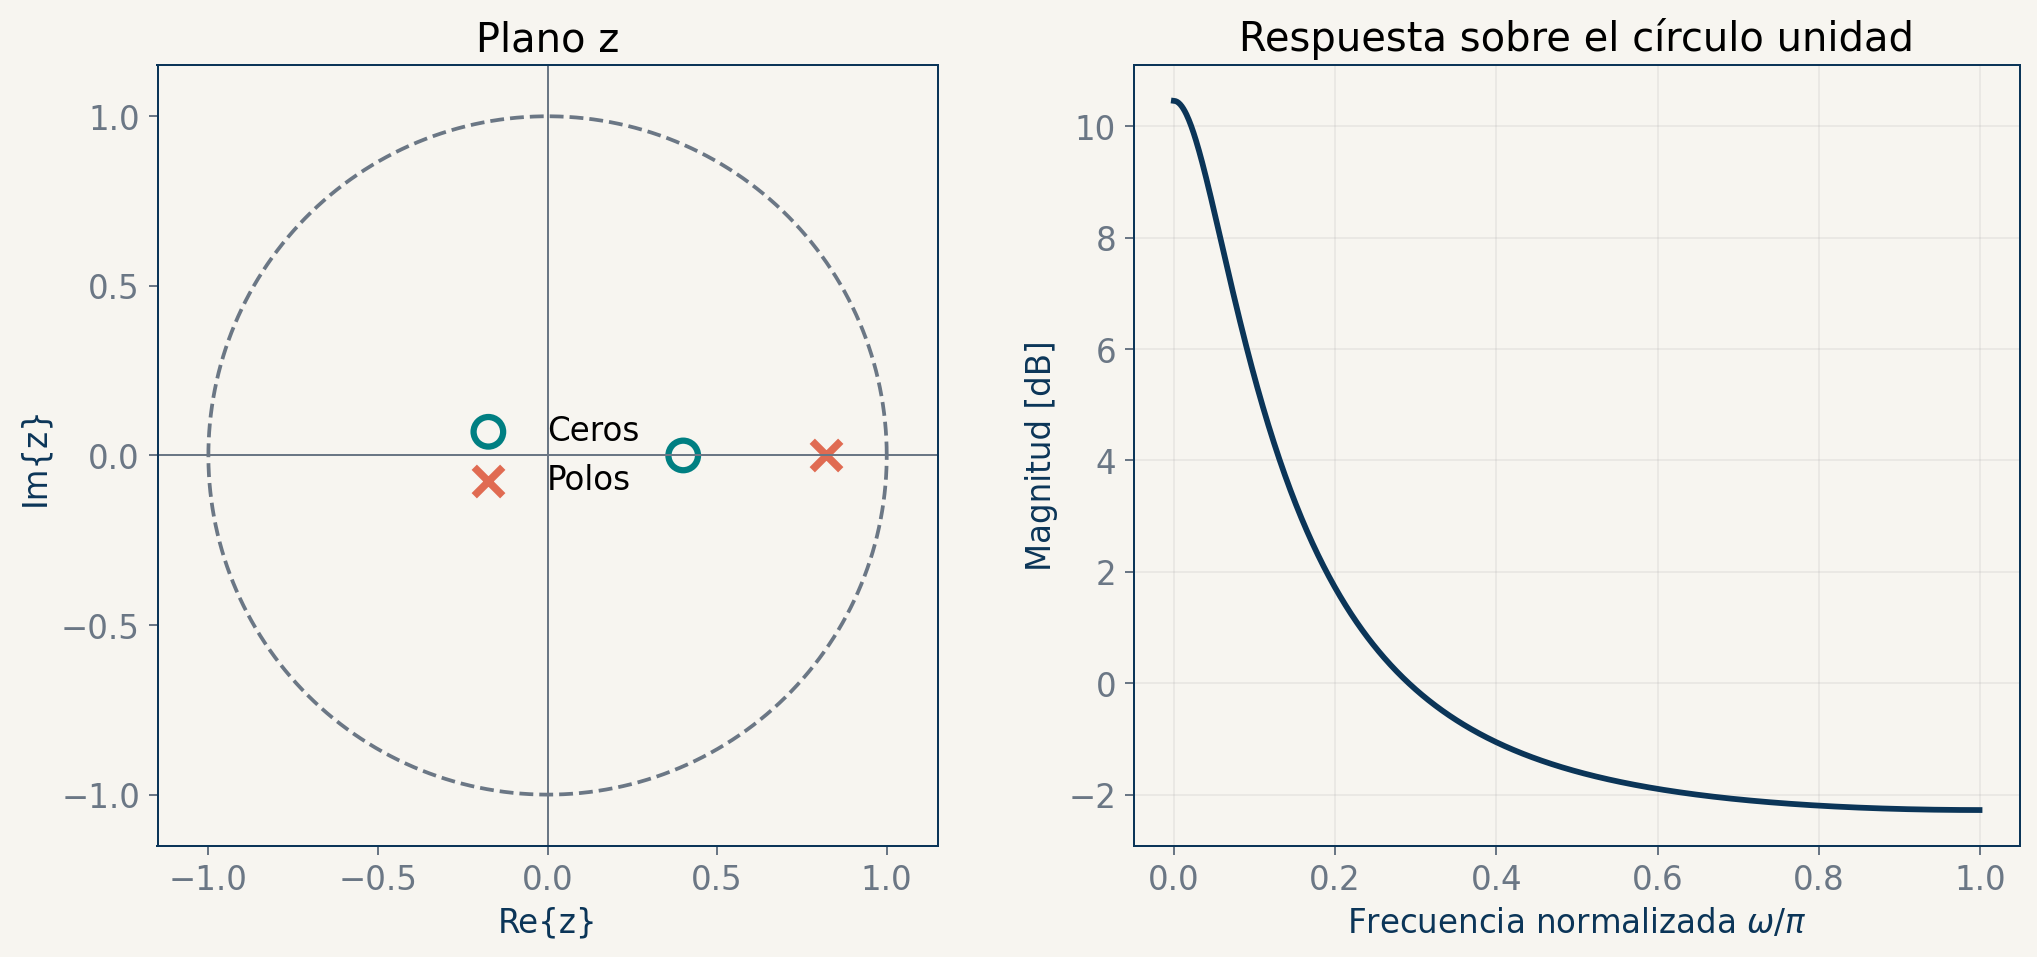
\includegraphics[width=0.83\linewidth,height=\textheight,keepaspectratio]{assets/pole_zero_response.png}

\begin{itemize}
\tightlist
\item
  Un cero cercano al círculo unidad atenúa frecuencias próximas a su
  ángulo.
\item
  Un polo cercano al círculo unidad realza y prolonga la respuesta.
\item
  La ganancia fija la escala global.
\end{itemize}

\begin{tcolorbox}[enhanced jigsaw, bottomrule=.15mm, opacitybacktitle=0.6, rightrule=.15mm, opacityback=0, left=2mm, leftrule=.75mm, title={Regla geométrica}, coltitle=black, colbacktitle=quarto-callout-note-color!10!white, toprule=.15mm, colframe=quarto-callout-note-color-frame, bottomtitle=1mm, toptitle=1mm, breakable, titlerule=0mm, arc=.35mm, colback=white]

\(|H(e^{j\omega})|\) depende de la razón entre distancias desde
\(e^{j\omega}\) a ceros y polos.

\end{tcolorbox}
\end{frame}

\begin{frame}{Estabilidad causal en sistemas racionales}
\phantomsection\label{estabilidad-causal-en-sistemas-racionales}
Para un sistema LTI racional:

\begin{itemize}
\tightlist
\item
  causalidad: ROC exterior al polo de mayor módulo;
\item
  estabilidad: la ROC incluye el círculo unidad;
\item
  causal y estable: todos los polos quedan dentro del círculo unidad.
\end{itemize}

\begin{tcolorbox}[enhanced jigsaw, bottomrule=.15mm, opacitybacktitle=0.6, rightrule=.15mm, opacityback=0, left=2mm, leftrule=.75mm, title={Matiz}, coltitle=black, colbacktitle=quarto-callout-warning-color!10!white, toprule=.15mm, colframe=quarto-callout-warning-color-frame, bottomtitle=1mm, toptitle=1mm, breakable, titlerule=0mm, arc=.35mm, colback=white]

``Polos dentro del círculo'' implica estabilidad solo después de fijar
la realización causal y descartar cancelaciones frágiles.

\end{tcolorbox}
\end{frame}

\begin{frame}{Propiedades operativas de la transformada Z}
\phantomsection\label{propiedades-operativas-de-la-transformada-z}
\begin{longtable}[]{@{}ll@{}}
\toprule\noalign{}
Operación en tiempo & Transformada \\
\midrule\noalign{}
\endhead
\(a x_1[n]+b x_2[n]\) & \(aX_1(z)+bX_2(z)\) \\
\(x[n-n_0]\) & \(z^{-n_0}X(z)\) \\
\(x[n]*h[n]\) & \(X(z)H(z)\) \\
\(a^n x[n]\) & \(X(z/a)\) \\
\bottomrule\noalign{}
\end{longtable}

\begin{tcolorbox}[enhanced jigsaw, bottomrule=.15mm, opacitybacktitle=0.6, rightrule=.15mm, opacityback=0, left=2mm, leftrule=.75mm, title={Puente}, coltitle=black, colbacktitle=quarto-callout-important-color!10!white, toprule=.15mm, colframe=quarto-callout-important-color-frame, bottomtitle=1mm, toptitle=1mm, breakable, titlerule=0mm, arc=.35mm, colback=white]

El desplazamiento se vuelve multiplicación por \(z^{-1}\); por eso los
retardos aparecen directamente en ecuaciones de filtros.

\end{tcolorbox}
\end{frame}

\begin{frame}{Verificación 9.1}
\phantomsection\label{verificaciuxf3n-9.1}
Para

\[
H(z)=\frac{1+z^{-1}}{1-1.1z^{-1}},
\]

\begin{enumerate}
\tightlist
\item
  ubique cero y polo;
\item
  evalúe estabilidad si la realización es causal;
\item
  explique por qué el cero en \(-1\) atenúa Nyquist.
\end{enumerate}

\begin{tcolorbox}[enhanced jigsaw, bottomrule=.15mm, opacitybacktitle=0.6, rightrule=.15mm, opacityback=0, left=2mm, leftrule=.75mm, title={Respuesta esperada}, coltitle=black, colbacktitle=quarto-callout-note-color!10!white, toprule=.15mm, colframe=quarto-callout-note-color-frame, bottomtitle=1mm, toptitle=1mm, breakable, titlerule=0mm, arc=.35mm, colback=white]

Cero \(z=-1\), polo \(z=1.1\). La realización causal no es estable. En
\(z=e^{j\pi}=-1\), el numerador se anula.

\end{tcolorbox}
\end{frame}

\begin{frame}{Cierre de la sesión 17}
\phantomsection\label{cierre-de-la-sesiuxf3n-17}
\begin{tcolorbox}[enhanced jigsaw, bottomrule=.15mm, opacitybacktitle=0.6, rightrule=.15mm, opacityback=0, left=2mm, leftrule=.75mm, title={Síntesis}, coltitle=black, colbacktitle=quarto-callout-important-color!10!white, toprule=.15mm, colframe=quarto-callout-important-color-frame, bottomtitle=1mm, toptitle=1mm, breakable, titlerule=0mm, arc=.35mm, colback=white]

La transformada Z incorpora convergencia y lateralidad. En sistemas
racionales causales, polos, ceros y círculo unidad permiten razonar
sobre respuesta frecuencial y estabilidad.

\end{tcolorbox}
\end{frame}

\section{Semana 9 · Sesión 2}\label{semana-9-sesiuxf3n-2}

\begin{frame}{Diseñar un FIR significa controlar el truncamiento}
\phantomsection\label{diseuxf1ar-un-fir-significa-controlar-el-truncamiento}
\textbf{Resultados de aprendizaje}

\begin{itemize}
\tightlist
\item
  Traducir un objetivo biomédico a especificaciones de filtro.
\item
  Diseñar un FIR por truncamiento y ventana.
\item
  Verificar magnitud, fase, retardo y efecto temporal.
\end{itemize}

\textbf{Pregunta de entrada:} ¿por qué el filtro ideal no puede
implementarse directamente?
\end{frame}

\begin{frame}{El diseño empieza con una especificación medible}
\phantomsection\label{el-diseuxf1o-empieza-con-una-especificaciuxf3n-medible}
\begin{longtable}[]{@{}ll@{}}
\toprule\noalign{}
Símbolo & Decisión \\
\midrule\noalign{}
\endhead
\(f_p\) & borde de banda pasante \\
\(f_{st}\) & borde de banda de rechazo \\
\(A_p\) & rizado o pérdida permitida \\
\(A_s\) & atenuación requerida \\
\(f_s\) & frecuencia de muestreo \\
fase/retardo & distorsión temporal tolerable \\
\bottomrule\noalign{}
\end{longtable}

\begin{tcolorbox}[enhanced jigsaw, bottomrule=.15mm, opacitybacktitle=0.6, rightrule=.15mm, opacityback=0, left=2mm, leftrule=.75mm, title={Concepto principal}, coltitle=black, colbacktitle=quarto-callout-important-color!10!white, toprule=.15mm, colframe=quarto-callout-important-color-frame, bottomtitle=1mm, toptitle=1mm, breakable, titlerule=0mm, arc=.35mm, colback=white]

``Quitar ruido'' no es una especificación. Debe indicar qué frecuencias
conservar, cuáles atenuar y cuánto error tolerar.

\end{tcolorbox}
\end{frame}

\begin{frame}{El pasa-bajas ideal tiene respuesta infinita y no causal}
\phantomsection\label{el-pasa-bajas-ideal-tiene-respuesta-infinita-y-no-causal}
\[
H_d(e^{j\omega})=
\begin{cases}
1,& |\omega|\le\omega_c,\\
0,& \omega_c<|\omega|\le\pi.
\end{cases}
\]

Su respuesta al impulso es una sinc:

\[
h_d[n]=\frac{\sin(\omega_c n)}{\pi n},
\qquad h_d[0]=\frac{\omega_c}{\pi}.
\]

\begin{tcolorbox}[enhanced jigsaw, bottomrule=.15mm, opacitybacktitle=0.6, rightrule=.15mm, opacityback=0, left=2mm, leftrule=.75mm, title={Limitación}, coltitle=black, colbacktitle=quarto-callout-warning-color!10!white, toprule=.15mm, colframe=quarto-callout-warning-color-frame, bottomtitle=1mm, toptitle=1mm, breakable, titlerule=0mm, arc=.35mm, colback=white]

\(h_d[n]\) se extiende hacia \(n=\pm\infty\). Se debe truncar y
desplazar para implementarla.

\end{tcolorbox}
\end{frame}

\begin{frame}{Ventanar controla el compromiso de truncamiento}
\phantomsection\label{ventanar-controla-el-compromiso-de-truncamiento}
\[
h[n]=h_d[n-M/2]w[n],\qquad 0\le n\le M.
\]

\begin{longtable}[]{@{}llll@{}}
\toprule\noalign{}
Ventana & Transición & Lóbulos laterales & Uso típico \\
\midrule\noalign{}
\endhead
Rectangular & Más estrecha & Altos & Exploración, poco rechazo \\
Hann/Hamming & Moderada & Menores & Compromiso general \\
Blackman & Más ancha & Mucho menores & Mayor atenuación \\
Kaiser & Ajustable & Ajustable & Diseño por especificaciones \\
\bottomrule\noalign{}
\end{longtable}

\begin{tcolorbox}[enhanced jigsaw, bottomrule=.15mm, opacitybacktitle=0.6, rightrule=.15mm, opacityback=0, left=2mm, leftrule=.75mm, title={Principio}, coltitle=black, colbacktitle=quarto-callout-note-color!10!white, toprule=.15mm, colframe=quarto-callout-note-color-frame, bottomtitle=1mm, toptitle=1mm, breakable, titlerule=0mm, arc=.35mm, colback=white]

Reducir fuga en rechazo suele ampliar la transición para un orden fijo.

\end{tcolorbox}
\end{frame}

\begin{frame}{Un FIR simétrico conserva forma mediante fase lineal}
\phantomsection\label{un-fir-simuxe9trico-conserva-forma-mediante-fase-lineal}
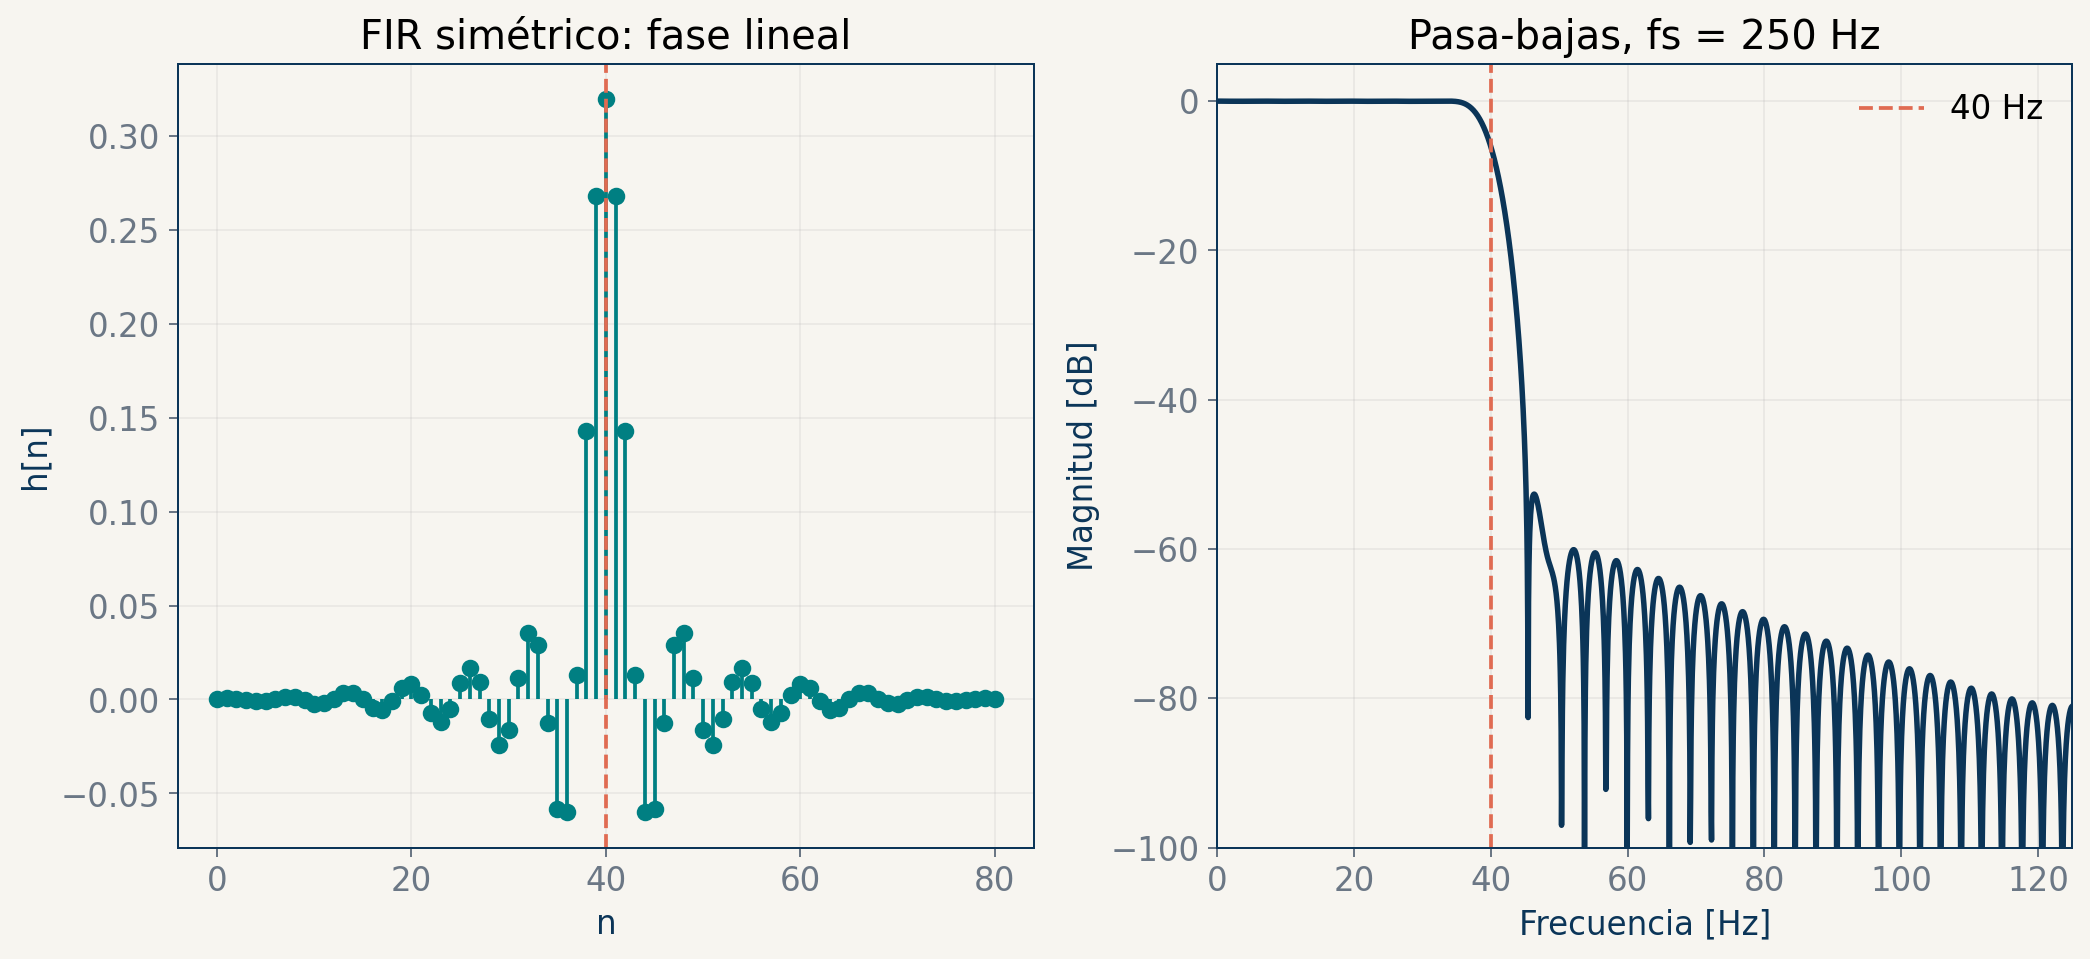
\includegraphics[width=0.83\linewidth,height=\textheight,keepaspectratio]{assets/fir_design.png}

Para un FIR simétrico de longitud \(L\), el retardo de grupo es
constante:

\[
\tau_g=\frac{L-1}{2}\ \text{muestras}.
\]

\begin{tcolorbox}[enhanced jigsaw, bottomrule=.15mm, opacitybacktitle=0.6, rightrule=.15mm, opacityback=0, left=2mm, leftrule=.75mm, title={Interpretación biomédica}, coltitle=black, colbacktitle=quarto-callout-important-color!10!white, toprule=.15mm, colframe=quarto-callout-important-color-frame, bottomtitle=1mm, toptitle=1mm, breakable, titlerule=0mm, arc=.35mm, colback=white]

La fase lineal preserva relaciones temporales internas, pero desplaza
toda la señal. En tiempo real, ese retardo puede ser crítico.

\end{tcolorbox}
\end{frame}

\begin{frame}{El orden se paga con transición y latencia}
\phantomsection\label{el-orden-se-paga-con-transiciuxf3n-y-latencia}
Al aumentar longitud del FIR:

\begin{itemize}
\tightlist
\item
  se estrecha la transición;
\item
  puede aumentar atenuación según ventana;
\item
  crece el costo computacional;
\item
  aumenta retardo lineal;
\item
  crecen efectos de borde.
\end{itemize}

\begin{tcolorbox}[enhanced jigsaw, bottomrule=.15mm, opacitybacktitle=0.6, rightrule=.15mm, opacityback=0, left=2mm, leftrule=.75mm, title={Decisión}, coltitle=black, colbacktitle=quarto-callout-warning-color!10!white, toprule=.15mm, colframe=quarto-callout-warning-color-frame, bottomtitle=1mm, toptitle=1mm, breakable, titlerule=0mm, arc=.35mm, colback=white]

No elija el orden por estética de la respuesta. Debe satisfacer
especificaciones con la menor complejidad compatible con el uso.

\end{tcolorbox}
\end{frame}

\begin{frame}[fragile]{Diseño FIR en Python}
\phantomsection\label{diseuxf1o-fir-en-python}
\begin{Shaded}
\begin{Highlighting}[]
\ImportTok{from}\NormalTok{ scipy }\ImportTok{import}\NormalTok{ signal}

\NormalTok{fs }\OperatorTok{=} \FloatTok{250.0}
\NormalTok{taps }\OperatorTok{=}\NormalTok{ signal.firwin(}
\NormalTok{    numtaps}\OperatorTok{=}\DecValTok{81}\NormalTok{,}
\NormalTok{    cutoff}\OperatorTok{=}\FloatTok{40.0}\NormalTok{,}
\NormalTok{    window}\OperatorTok{=}\StringTok{"hamming"}\NormalTok{,}
\NormalTok{    pass\_zero}\OperatorTok{=}\StringTok{"lowpass"}\NormalTok{,}
\NormalTok{    fs}\OperatorTok{=}\NormalTok{fs,}
\NormalTok{)}
\NormalTok{f, h }\OperatorTok{=}\NormalTok{ signal.freqz(taps, worN}\OperatorTok{=}\DecValTok{4096}\NormalTok{, fs}\OperatorTok{=}\NormalTok{fs)}
\end{Highlighting}
\end{Shaded}

\begin{tcolorbox}[enhanced jigsaw, bottomrule=.15mm, opacitybacktitle=0.6, rightrule=.15mm, opacityback=0, left=2mm, leftrule=.75mm, title={Buena práctica}, coltitle=black, colbacktitle=quarto-callout-tip-color!10!white, toprule=.15mm, colframe=quarto-callout-tip-color-frame, bottomtitle=1mm, toptitle=1mm, breakable, titlerule=0mm, arc=.35mm, colback=white]

Use \texttt{fs=} para expresar bordes en Hz y reduzca errores de
normalización respecto a Nyquist.

\end{tcolorbox}
\end{frame}

\begin{frame}{Aplicar no equivale a validar}
\phantomsection\label{aplicar-no-equivale-a-validar}
Una validación mínima incluye:

\begin{enumerate}
\tightlist
\item
  respuesta en magnitud con \(A_p\) y \(A_s\);
\item
  fase y retardo de grupo;
\item
  respuesta al impulso y estabilidad numérica;
\item
  señal de prueba con componentes conocidas;
\item
  inspección temporal del evento biomédico;
\item
  análisis de bordes y transitorios.
\end{enumerate}

\begin{tcolorbox}[enhanced jigsaw, bottomrule=.15mm, opacitybacktitle=0.6, rightrule=.15mm, opacityback=0, left=2mm, leftrule=.75mm, title={Criterio}, coltitle=black, colbacktitle=quarto-callout-important-color!10!white, toprule=.15mm, colframe=quarto-callout-important-color-frame, bottomtitle=1mm, toptitle=1mm, breakable, titlerule=0mm, arc=.35mm, colback=white]

La figura de la señal filtrada es evidencia insuficiente si no se
verifica que las especificaciones fueron satisfechas.

\end{tcolorbox}
\end{frame}

\begin{frame}[fragile]{\texttt{lfilter}, \texttt{filtfilt} y convolución
cambian la interpretación}
\phantomsection\label{lfilter-filtfilt-y-convoluciuxf3n-cambian-la-interpretaciuxf3n}
\begin{longtable}[]{@{}
  >{\raggedright\arraybackslash}p{(\linewidth - 6\tabcolsep) * \real{0.2143}}
  >{\centering\arraybackslash}p{(\linewidth - 6\tabcolsep) * \real{0.3571}}
  >{\raggedright\arraybackslash}p{(\linewidth - 6\tabcolsep) * \real{0.2143}}
  >{\raggedright\arraybackslash}p{(\linewidth - 6\tabcolsep) * \real{0.2143}}@{}}
\toprule\noalign{}
\begin{minipage}[b]{\linewidth}\raggedright
Método
\end{minipage} & \begin{minipage}[b]{\linewidth}\centering
Causal
\end{minipage} & \begin{minipage}[b]{\linewidth}\raggedright
Fase
\end{minipage} & \begin{minipage}[b]{\linewidth}\raggedright
Longitud/efectos
\end{minipage} \\
\midrule\noalign{}
\endhead
\texttt{np.convolve(...,\ full)} & Depende de \(h\) & La del FIR &
Longitud completa \\
\texttt{signal.lfilter} & Sí & La del filtro & Estado inicial y
transitorio \\
\texttt{signal.filtfilt} & No & Fase neta cero & Orden efectivo y bordes
cambian \\
\bottomrule\noalign{}
\end{longtable}

\begin{tcolorbox}[enhanced jigsaw, bottomrule=.15mm, opacitybacktitle=0.6, rightrule=.15mm, opacityback=0, left=2mm, leftrule=.75mm, title={Reproducibilidad}, coltitle=black, colbacktitle=quarto-callout-warning-color!10!white, toprule=.15mm, colframe=quarto-callout-warning-color-frame, bottomtitle=1mm, toptitle=1mm, breakable, titlerule=0mm, arc=.35mm, colback=white]

Documente función, modo, relleno de bordes y si se compensó el retardo.
El mismo vector de coeficientes puede producir salidas alineadas de
forma distinta.

\end{tcolorbox}
\end{frame}

\begin{frame}{Cierre de la semana 9}
\phantomsection\label{cierre-de-la-semana-9}
\begin{itemize}
\tightlist
\item
  La ROC completa el significado de \(X(z)\).
\item
  \(H(z)\) conecta ecuación en diferencias, polos, ceros e impulso.
\item
  Un FIR puede ofrecer estabilidad inherente y fase lineal.
\item
  La ventana gobierna transición y lóbulos laterales.
\end{itemize}

\begin{tcolorbox}[enhanced jigsaw, bottomrule=.15mm, opacitybacktitle=0.6, rightrule=.15mm, opacityback=0, left=2mm, leftrule=.75mm, title={Puente a la semana 10}, coltitle=black, colbacktitle=quarto-callout-important-color!10!white, toprule=.15mm, colframe=quarto-callout-important-color-frame, bottomtitle=1mm, toptitle=1mm, breakable, titlerule=0mm, arc=.35mm, colback=white]

Los IIR satisfacen transiciones exigentes con menos coeficientes, pero
exigen controlar estabilidad, fase y precisión numérica.

\end{tcolorbox}

Apoyo: Esakkirajan, Veerakumar y Subudhi (2024), caps. 5 y 7,
doi:10.1007/978-981-99-6752-0.
\end{frame}

\section{Semana 10 · Sesión 1}\label{semana-10-sesiuxf3n-1}

\begin{frame}{Un IIR traduce especificaciones en polos y ceros}
\phantomsection\label{un-iir-traduce-especificaciones-en-polos-y-ceros}
\textbf{Resultados de aprendizaje}

\begin{itemize}
\tightlist
\item
  Comparar FIR e IIR según magnitud, fase, orden y estabilidad.
\item
  Explicar prototipos analógicos y transformación bilineal.
\item
  Diseñar un Butterworth digital con especificaciones explícitas.
\end{itemize}

\textbf{Pregunta de entrada:} ¿un menor orden hace automáticamente mejor
a un IIR?
\end{frame}

\begin{frame}{FIR e IIR resuelven compromisos diferentes}
\phantomsection\label{fir-e-iir-resuelven-compromisos-diferentes}
\begin{longtable}[]{@{}lll@{}}
\toprule\noalign{}
Criterio & FIR & IIR \\
\midrule\noalign{}
\endhead
Respuesta al impulso & Finita & Teóricamente infinita \\
Realimentación & No necesaria & Sí \\
Fase lineal exacta & Posible & No, salvo casos triviales \\
Orden para transición dada & Mayor & Menor \\
Estabilidad & Inherente si coeficientes finitos & Depende de polos \\
Sensibilidad numérica & Menor & Mayor, especialmente en orden alto \\
\bottomrule\noalign{}
\end{longtable}

\begin{tcolorbox}[enhanced jigsaw, bottomrule=.15mm, opacitybacktitle=0.6, rightrule=.15mm, opacityback=0, left=2mm, leftrule=.75mm, title={Decisión}, coltitle=black, colbacktitle=quarto-callout-important-color!10!white, toprule=.15mm, colframe=quarto-callout-important-color-frame, bottomtitle=1mm, toptitle=1mm, breakable, titlerule=0mm, arc=.35mm, colback=white]

La elección depende de fase, latencia, recursos, estabilidad y
especificaciones; no de una superioridad universal.

\end{tcolorbox}
\end{frame}

\begin{frame}{Un prototipo analógico define la forma de magnitud}
\phantomsection\label{un-prototipo-analuxf3gico-define-la-forma-de-magnitud}
Familias clásicas:

\begin{itemize}
\tightlist
\item
  \textbf{Butterworth:} magnitud máximamente plana en banda pasante.
\item
  \textbf{Chebyshev I:} rizado permitido en pasante, transición más
  rápida.
\item
  \textbf{Chebyshev II:} rizado en rechazo.
\item
  \textbf{Elíptico:} rizado en ambas bandas, mínimo orden frecuente.
\end{itemize}

\begin{tcolorbox}[enhanced jigsaw, bottomrule=.15mm, opacitybacktitle=0.6, rightrule=.15mm, opacityback=0, left=2mm, leftrule=.75mm, title={Selección didáctica}, coltitle=black, colbacktitle=quarto-callout-note-color!10!white, toprule=.15mm, colframe=quarto-callout-note-color-frame, bottomtitle=1mm, toptitle=1mm, breakable, titlerule=0mm, arc=.35mm, colback=white]

Butterworth permite estudiar un diseño sin introducir rizado deliberado
en la banda de EMG que se desea conservar.

\end{tcolorbox}
\end{frame}

\begin{frame}{La transformación bilineal evita aliasing de polos}
\phantomsection\label{la-transformaciuxf3n-bilineal-evita-aliasing-de-polos}
\[
s=\frac{2f_s(1-z^{-1})}{1+z^{-1}}.
\]

Mapea:

\begin{itemize}
\tightlist
\item
  semiplano izquierdo de \(s\) al interior del círculo unidad;
\item
  eje \(j\Omega\) al círculo unidad;
\item
  todo el eje analógico en \(-\pi<\omega<\pi\).
\end{itemize}

\begin{tcolorbox}[enhanced jigsaw, bottomrule=.15mm, opacitybacktitle=0.6, rightrule=.15mm, opacityback=0, left=2mm, leftrule=.75mm, title={Consecuencia}, coltitle=black, colbacktitle=quarto-callout-important-color!10!white, toprule=.15mm, colframe=quarto-callout-important-color-frame, bottomtitle=1mm, toptitle=1mm, breakable, titlerule=0mm, arc=.35mm, colback=white]

Preserva estabilidad, pero deforma no linealmente el eje de frecuencias.

\end{tcolorbox}
\end{frame}

\begin{frame}{Predeformar corrige los bordes críticos}
\phantomsection\label{predeformar-corrige-los-bordes-cruxedticos}
La relación entre frecuencia digital \(f_d\) y analógica predeformada es

\[
\Omega=2f_s\tan\left(\pi\frac{f_d}{f_s}\right).
\]

No existe una escala lineal global entre ambos ejes.

\begin{tcolorbox}[enhanced jigsaw, bottomrule=.15mm, opacitybacktitle=0.6, rightrule=.15mm, opacityback=0, left=2mm, leftrule=.75mm, title={Error frecuente}, coltitle=black, colbacktitle=quarto-callout-warning-color!10!white, toprule=.15mm, colframe=quarto-callout-warning-color-frame, bottomtitle=1mm, toptitle=1mm, breakable, titlerule=0mm, arc=.35mm, colback=white]

Diseñar el prototipo con \(\Omega=2\pi f_d\) y aplicar bilineal desplaza
los bordes, especialmente cerca de Nyquist.

\end{tcolorbox}
\end{frame}

\begin{frame}{Butterworth distribuye polos para una magnitud plana}
\phantomsection\label{butterworth-distribuye-polos-para-una-magnitud-plana}
Para un pasa-bajas normalizado:

\[
|H(j\Omega)|^2=\frac{1}{1+(\Omega/\Omega_c)^{2N}}.
\]

Características:

\begin{itemize}
\tightlist
\item
  sin rizado en pasante;
\item
  pendiente creciente con el orden \(N\);
\item
  fase no lineal;
\item
  polos ubicados en el semiplano izquierdo del prototipo estable.
\end{itemize}

\begin{tcolorbox}[enhanced jigsaw, bottomrule=.15mm, opacitybacktitle=0.6, rightrule=.15mm, opacityback=0, left=2mm, leftrule=.75mm, title={Interpretación}, coltitle=black, colbacktitle=quarto-callout-note-color!10!white, toprule=.15mm, colframe=quarto-callout-note-color-frame, bottomtitle=1mm, toptitle=1mm, breakable, titlerule=0mm, arc=.35mm, colback=white]

``Máximamente plano'' describe magnitud cerca de DC; no significa fase
lineal ni respuesta transitoria óptima.

\end{tcolorbox}
\end{frame}

\begin{frame}{El orden se deriva de tolerancias, no se adivina}
\phantomsection\label{el-orden-se-deriva-de-tolerancias-no-se-adivina}
Para un prototipo pasa-bajas:

\[
N\ge
\frac{
\log_{10}\!\left(\dfrac{10^{A_s/10}-1}{10^{A_p/10}-1}\right)
}{
2\log_{10}(\Omega_s/\Omega_p)
}.
\]

Luego se redondea hacia arriba.

\begin{tcolorbox}[enhanced jigsaw, bottomrule=.15mm, opacitybacktitle=0.6, rightrule=.15mm, opacityback=0, left=2mm, leftrule=.75mm, title={Lectura}, coltitle=black, colbacktitle=quarto-callout-important-color!10!white, toprule=.15mm, colframe=quarto-callout-important-color-frame, bottomtitle=1mm, toptitle=1mm, breakable, titlerule=0mm, arc=.35mm, colback=white]

Transición más estrecha o mayor atenuación exigen orden mayor. El costo
nace de la especificación.

\end{tcolorbox}
\end{frame}

\begin{frame}{Diseñar en SOS mejora robustez numérica}
\phantomsection\label{diseuxf1ar-en-sos-mejora-robustez-numuxe9rica}
Un IIR de orden alto en forma polinómica directa puede ser sensible al
redondeo.

\[
H(z)=\prod_{m=1}^{K}
\frac{b_{0m}+b_{1m}z^{-1}+b_{2m}z^{-2}}
{a_{0m}+a_{1m}z^{-1}+a_{2m}z^{-2}}.
\]

\begin{tcolorbox}[enhanced jigsaw, bottomrule=.15mm, opacitybacktitle=0.6, rightrule=.15mm, opacityback=0, left=2mm, leftrule=.75mm, title={Buena práctica}, coltitle=black, colbacktitle=quarto-callout-important-color!10!white, toprule=.15mm, colframe=quarto-callout-important-color-frame, bottomtitle=1mm, toptitle=1mm, breakable, titlerule=0mm, arc=.35mm, colback=white]

Implemente como secciones de segundo orden (SOS), especialmente en
pasabandas y órdenes moderados o altos.

\end{tcolorbox}
\end{frame}

\begin{frame}[fragile]{Código de diseño IIR reproducible}
\phantomsection\label{cuxf3digo-de-diseuxf1o-iir-reproducible}
\begin{Shaded}
\begin{Highlighting}[]
\ImportTok{from}\NormalTok{ scipy }\ImportTok{import}\NormalTok{ signal}

\NormalTok{fs }\OperatorTok{=} \FloatTok{2000.0}
\NormalTok{wp }\OperatorTok{=}\NormalTok{ [}\FloatTok{20.0}\NormalTok{, }\FloatTok{450.0}\NormalTok{]}
\NormalTok{ws }\OperatorTok{=}\NormalTok{ [}\FloatTok{10.0}\NormalTok{, }\FloatTok{550.0}\NormalTok{]}
\NormalTok{gpass, gstop }\OperatorTok{=} \FloatTok{1.0}\NormalTok{, }\FloatTok{40.0}

\NormalTok{order, wn }\OperatorTok{=}\NormalTok{ signal.buttord(wp, ws, gpass, gstop, fs}\OperatorTok{=}\NormalTok{fs)}
\NormalTok{sos }\OperatorTok{=}\NormalTok{ signal.butter(order, wn, btype}\OperatorTok{=}\StringTok{"bandpass"}\NormalTok{, fs}\OperatorTok{=}\NormalTok{fs,}
\NormalTok{                    output}\OperatorTok{=}\StringTok{"sos"}\NormalTok{)}
\end{Highlighting}
\end{Shaded}

\begin{tcolorbox}[enhanced jigsaw, bottomrule=.15mm, opacitybacktitle=0.6, rightrule=.15mm, opacityback=0, left=2mm, leftrule=.75mm, title={Verificación necesaria}, coltitle=black, colbacktitle=quarto-callout-warning-color!10!white, toprule=.15mm, colframe=quarto-callout-warning-color-frame, bottomtitle=1mm, toptitle=1mm, breakable, titlerule=0mm, arc=.35mm, colback=white]

\texttt{wn} es la frecuencia crítica devuelta por el diseño; no debe
suponerse idéntica a los bordes iniciales sin revisar la respuesta.

\end{tcolorbox}
\end{frame}

\begin{frame}{Verificación 10.1}
\phantomsection\label{verificaciuxf3n-10.1}
Un diseñador cambia \(f_s\) de 2000 a 1000 Hz y conserva \(f_H=450\) Hz.

\begin{enumerate}
\tightlist
\item
  ¿Qué ocurre con el margen hasta Nyquist?
\item
  ¿Cómo cambia la dificultad de la transición superior?
\item
  ¿Por qué podría aumentar el orden o fallar la especificación?
\end{enumerate}

\begin{tcolorbox}[enhanced jigsaw, bottomrule=.15mm, opacitybacktitle=0.6, rightrule=.15mm, opacityback=0, left=2mm, leftrule=.75mm, title={Respuesta esperada}, coltitle=black, colbacktitle=quarto-callout-note-color!10!white, toprule=.15mm, colframe=quarto-callout-note-color-frame, bottomtitle=1mm, toptitle=1mm, breakable, titlerule=0mm, arc=.35mm, colback=white]

Nyquist baja de 1000 a 500 Hz; solo quedan 50 Hz de margen. La
transición se vuelve mucho más exigente y sensible a predeformación y
orden.

\end{tcolorbox}
\end{frame}

\begin{frame}{Cierre de la sesión 19}
\phantomsection\label{cierre-de-la-sesiuxf3n-19}
\begin{tcolorbox}[enhanced jigsaw, bottomrule=.15mm, opacitybacktitle=0.6, rightrule=.15mm, opacityback=0, left=2mm, leftrule=.75mm, title={Síntesis}, coltitle=black, colbacktitle=quarto-callout-important-color!10!white, toprule=.15mm, colframe=quarto-callout-important-color-frame, bottomtitle=1mm, toptitle=1mm, breakable, titlerule=0mm, arc=.35mm, colback=white]

El prototipo fija la forma de magnitud, la transformación bilineal
preserva estabilidad y deforma frecuencia, y las SOS reducen
sensibilidad numérica.

\end{tcolorbox}
\end{frame}

\section{Semana 10 · Sesión 2}\label{semana-10-sesiuxf3n-2}

\begin{frame}{Un pasabanda para EMG debe justificarse y validarse}
\phantomsection\label{un-pasabanda-para-emg-debe-justificarse-y-validarse}
\textbf{Resultados de aprendizaje}

\begin{itemize}
\tightlist
\item
  Relacionar fisiología, artefactos y banda de diseño.
\item
  Comparar filtrado causal y de fase neta cero.
\item
  Validar respuesta frecuencial y efecto sobre una señal sintética.
\end{itemize}

\textbf{Pregunta de entrada:} ¿un pasabanda 20-450 Hz es una regla
universal para EMG?
\end{frame}

\begin{frame}{La EMG superficial es una suma interferencial}
\phantomsection\label{la-emg-superficial-es-una-suma-interferencial}
El registro combina potenciales de acción de múltiples unidades motoras,
conducción volumétrica y respuesta del montaje.

\begin{itemize}
\tightlist
\item
  La actividad no es una única sinusoide.
\item
  Tejidos y geometría modifican amplitud y espectro.
\item
  Contracción, fatiga, músculo y protocolo cambian el registro.
\item
  Movimiento y otras fuentes fisiológicas pueden solaparse.
\end{itemize}

\begin{tcolorbox}[enhanced jigsaw, bottomrule=.15mm, opacitybacktitle=0.6, rightrule=.15mm, opacityback=0, left=2mm, leftrule=.75mm, title={Concepto principal}, coltitle=black, colbacktitle=quarto-callout-important-color!10!white, toprule=.15mm, colframe=quarto-callout-important-color-frame, bottomtitle=1mm, toptitle=1mm, breakable, titlerule=0mm, arc=.35mm, colback=white]

La banda útil no es una propiedad universal de ``la EMG''. Se justifica
para un montaje, tarea, sensor, \(f_s\) y objetivo de análisis.

\end{tcolorbox}

Contexto fisiológico y de medición: Kaniusas (2019),
doi:10.1007/978-3-319-74917-4.
\end{frame}

\begin{frame}{Especificación didáctica del caso}
\phantomsection\label{especificaciuxf3n-diduxe1ctica-del-caso}
\textbf{Objetivo:} conservar actividad muscular útil y atenuar deriva,
movimiento y contenido muy alto.

\begin{longtable}[]{@{}lrr@{}}
\toprule\noalign{}
Región & Borde propuesto & Tolerancia \\
\midrule\noalign{}
\endhead
Rechazo inferior & \(0-10\) Hz & al menos 40 dB \\
Transición inferior & \(10-20\) Hz & - \\
Pasante & \(20-450\) Hz & pérdida menor a 1 dB \\
Transición superior & \(450-550\) Hz & - \\
Rechazo superior & \(550-1000\) Hz & al menos 40 dB \\
\bottomrule\noalign{}
\end{longtable}

\begin{tcolorbox}[enhanced jigsaw, bottomrule=.15mm, opacitybacktitle=0.6, rightrule=.15mm, opacityback=0, left=2mm, leftrule=.75mm, title={Alcance}, coltitle=black, colbacktitle=quarto-callout-warning-color!10!white, toprule=.15mm, colframe=quarto-callout-warning-color-frame, bottomtitle=1mm, toptitle=1mm, breakable, titlerule=0mm, arc=.35mm, colback=white]

Son especificaciones docentes, no una recomendación clínica ni un
estándar universal.

\end{tcolorbox}
\end{frame}

\begin{frame}{El resultado debe verse en tiempo y frecuencia}
\phantomsection\label{el-resultado-debe-verse-en-tiempo-y-frecuencia}
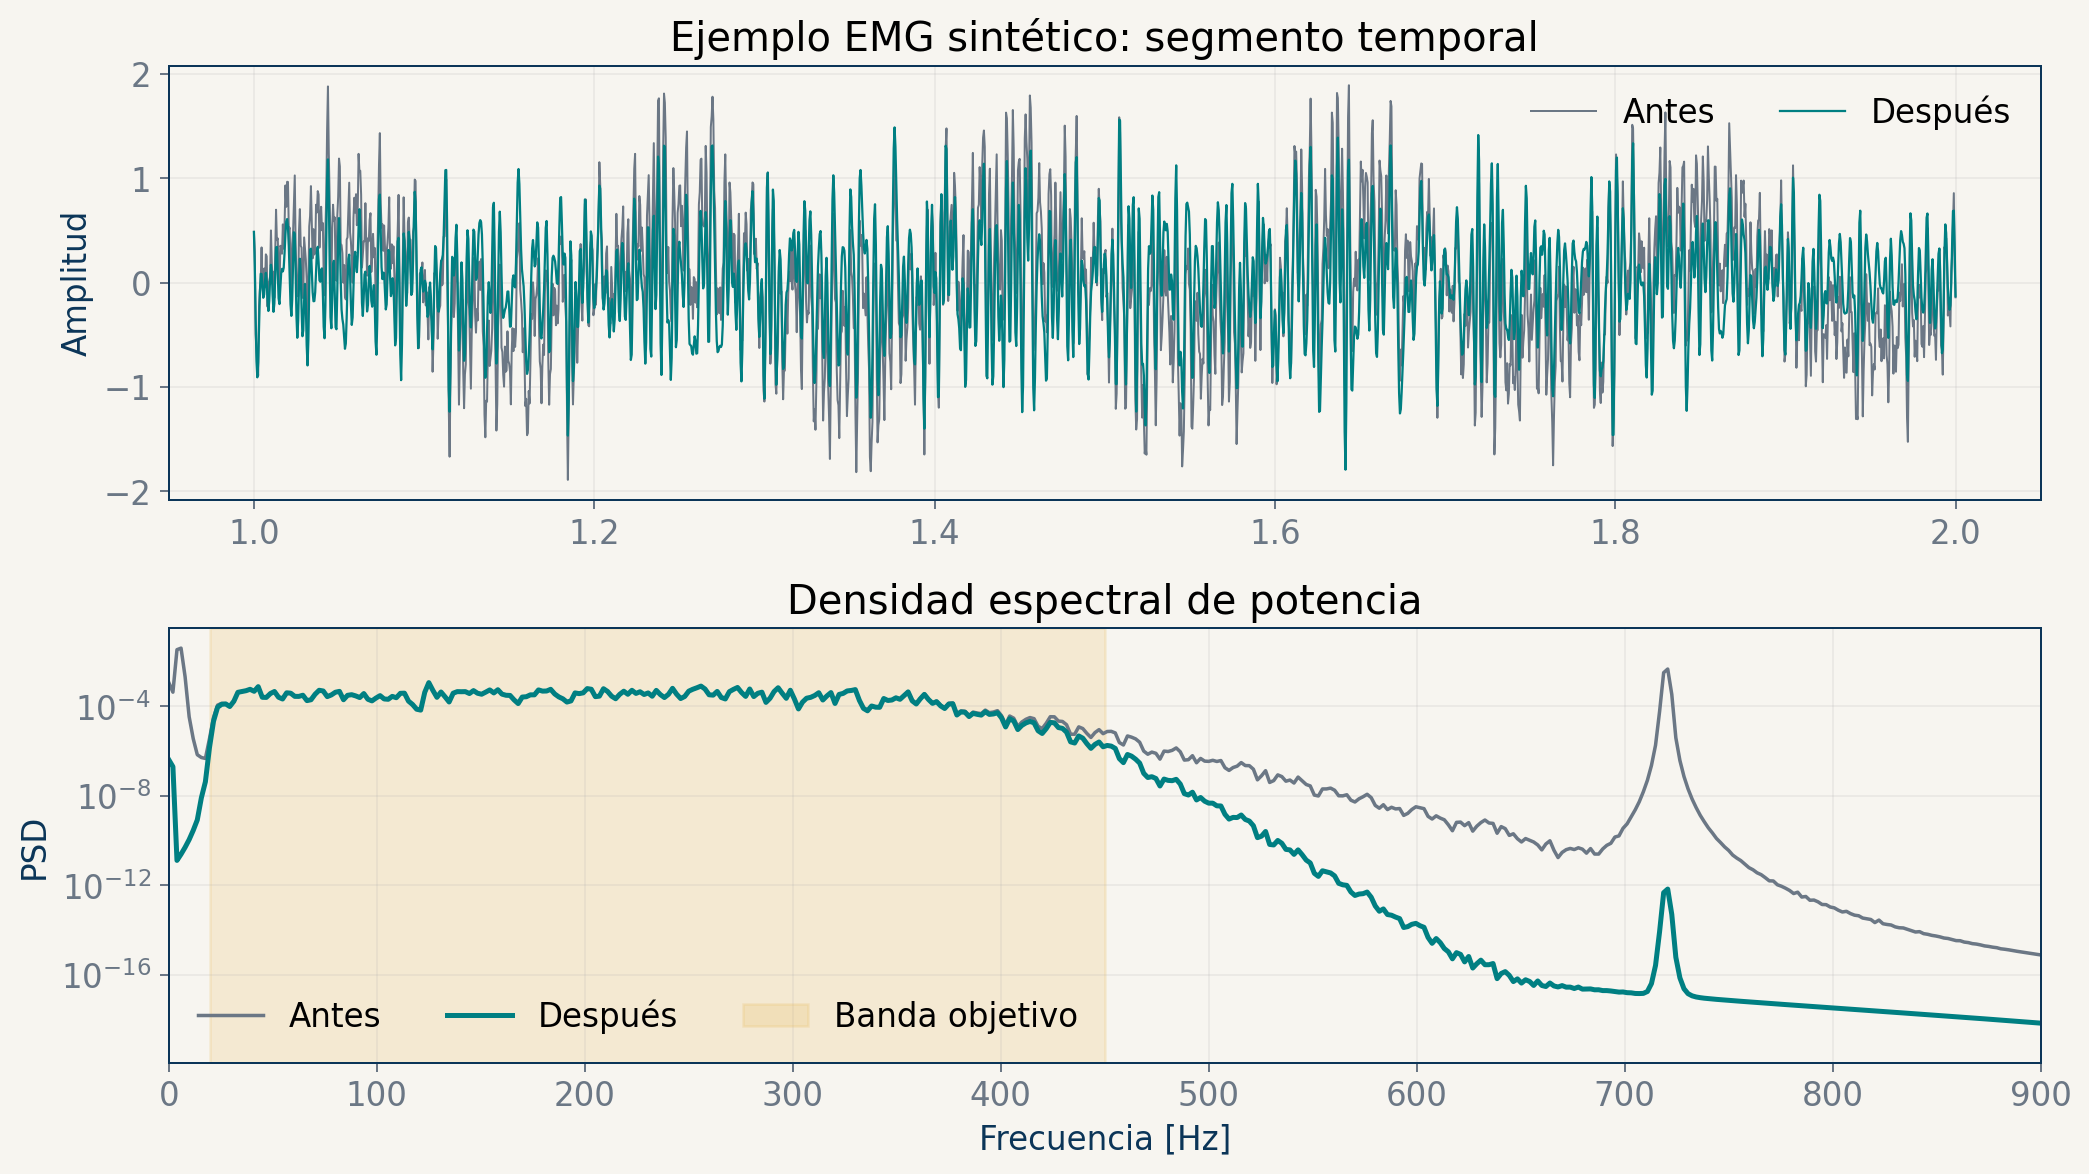
\includegraphics[width=0.86\linewidth,height=\textheight,keepaspectratio]{assets/iir_emg.png}

La señal y las contaminaciones son \textbf{sintéticas} y se usan para
probar el comportamiento conocido del filtro.

\begin{tcolorbox}[enhanced jigsaw, bottomrule=.15mm, opacitybacktitle=0.6, rightrule=.15mm, opacityback=0, left=2mm, leftrule=.75mm, title={Lectura}, coltitle=black, colbacktitle=quarto-callout-note-color!10!white, toprule=.15mm, colframe=quarto-callout-note-color-frame, bottomtitle=1mm, toptitle=1mm, breakable, titlerule=0mm, arc=.35mm, colback=white]

La PSD confirma atenuación de la deriva y de la componente alta. La
inspección temporal evalúa si la actividad transitoria sigue siendo
reconocible.

\end{tcolorbox}
\end{frame}

\begin{frame}{Causal y fase neta cero responden a preguntas distintas}
\phantomsection\label{causal-y-fase-neta-cero-responden-a-preguntas-distintas}
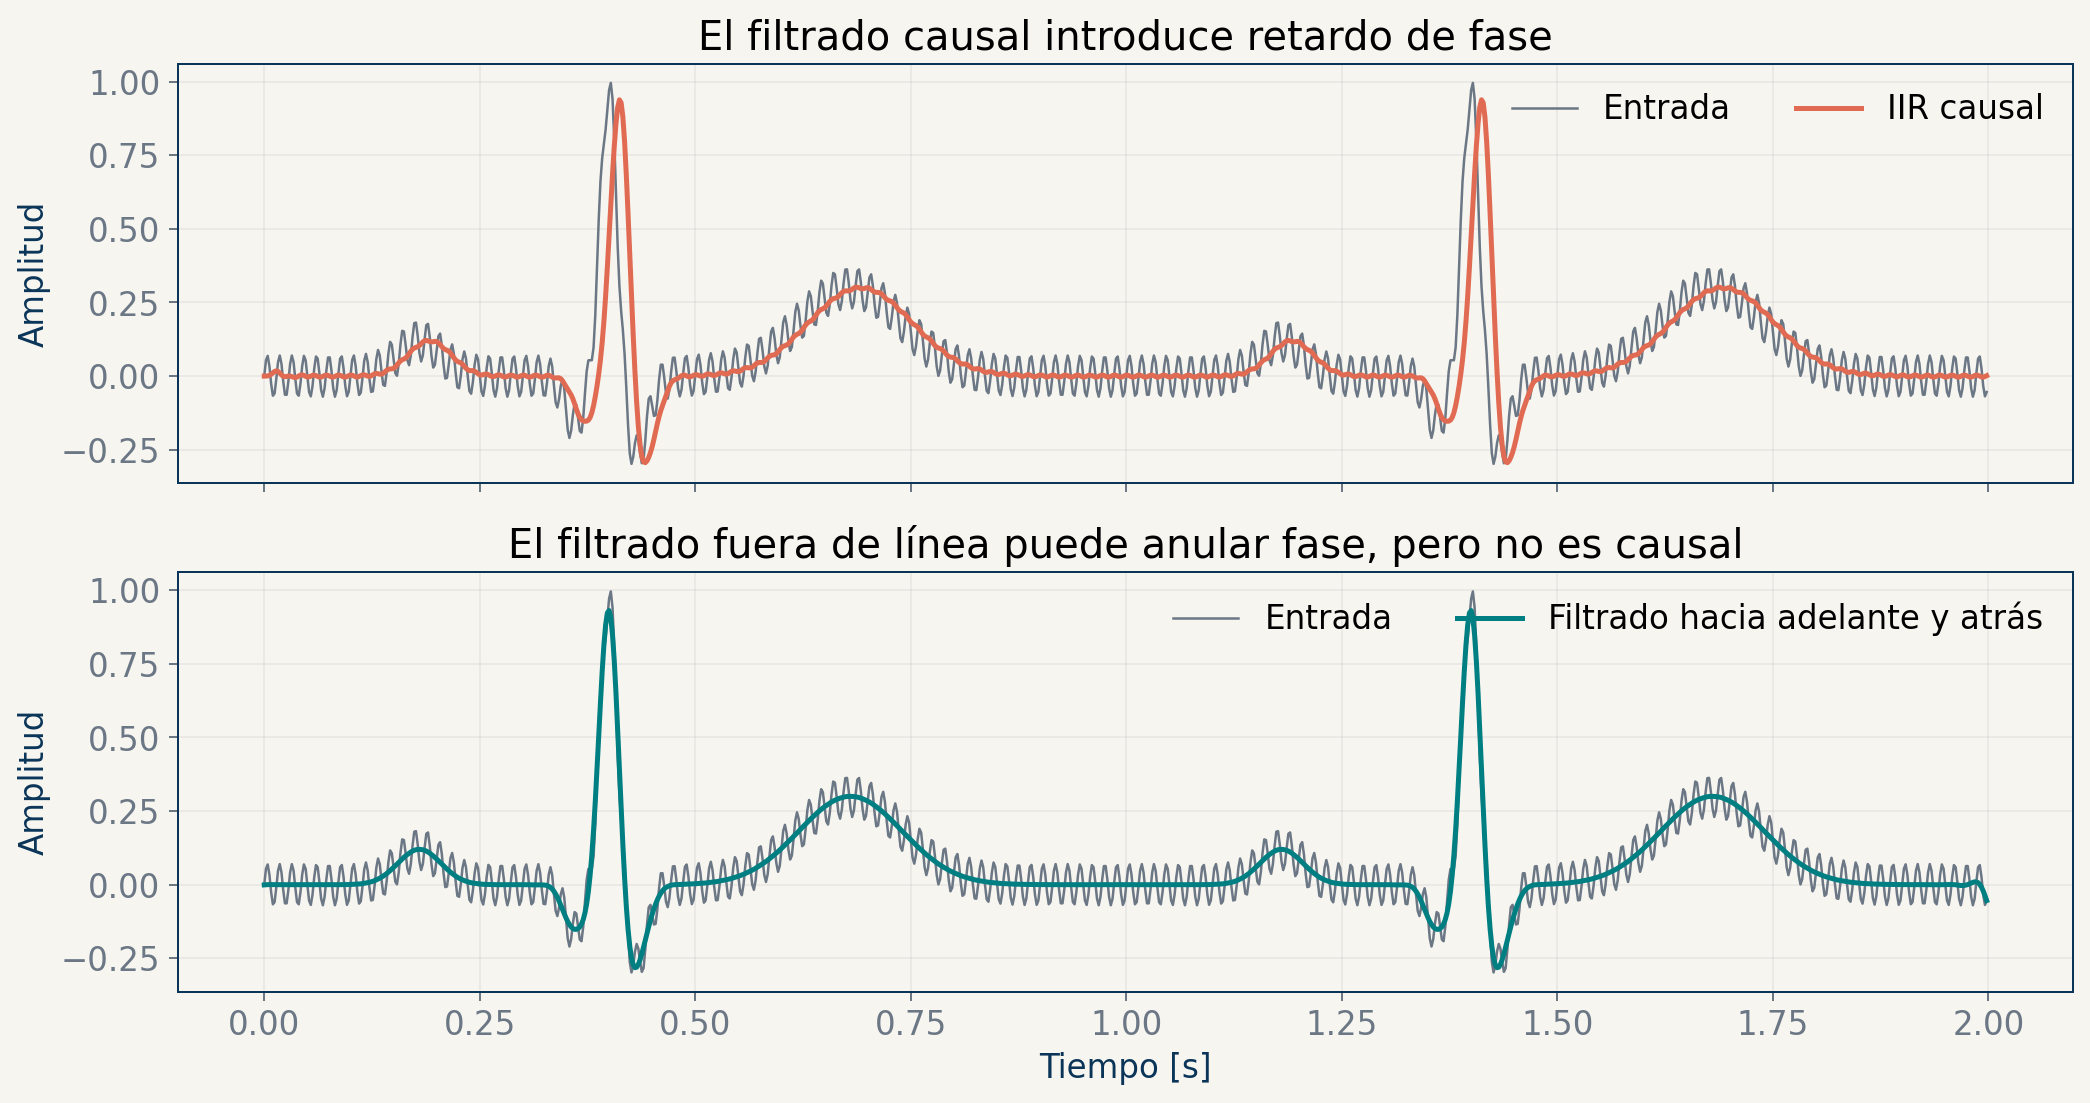
\includegraphics[width=0.85\linewidth,height=\textheight,keepaspectratio]{assets/phase_comparison.png}

\begin{tcolorbox}[enhanced jigsaw, bottomrule=.15mm, opacitybacktitle=0.6, rightrule=.15mm, opacityback=0, left=2mm, leftrule=.75mm, title={Decisión}, coltitle=black, colbacktitle=quarto-callout-important-color!10!white, toprule=.15mm, colframe=quarto-callout-important-color-frame, bottomtitle=1mm, toptitle=1mm, breakable, titlerule=0mm, arc=.35mm, colback=white]

Use filtrado causal para tiempo real. Use filtrado hacia adelante y
atrás solo fuera de línea, declarando efectos de borde y el cambio de
magnitud efectiva.

\end{tcolorbox}
\end{frame}

\begin{frame}[fragile]{\texttt{filtfilt} no es ``el mismo filtro sin
retardo''}
\phantomsection\label{filtfilt-no-es-el-mismo-filtro-sin-retardo}
Al aplicar hacia adelante y atrás:

\[
H_{ff}(e^{j\omega})=H(e^{j\omega})H^*(e^{j\omega})
=|H(e^{j\omega})|^2.
\]

Por tanto:

\begin{itemize}
\tightlist
\item
  la fase neta es cero;
\item
  el orden efectivo en magnitud se duplica;
\item
  la respuesta de magnitud cambia;
\item
  se requieren decisiones de padding y longitud mínima.
\end{itemize}

\begin{tcolorbox}[enhanced jigsaw, bottomrule=.15mm, opacitybacktitle=0.6, rightrule=.15mm, opacityback=0, left=2mm, leftrule=.75mm, title={Error frecuente}, coltitle=black, colbacktitle=quarto-callout-warning-color!10!white, toprule=.15mm, colframe=quarto-callout-warning-color-frame, bottomtitle=1mm, toptitle=1mm, breakable, titlerule=0mm, arc=.35mm, colback=white]

Comparar \texttt{sosfilt} y \texttt{sosfiltfilt} como si solo difirieran
en alineación temporal.

\end{tcolorbox}
\end{frame}

\begin{frame}{Un notch de red no debe añadirse automáticamente}
\phantomsection\label{un-notch-de-red-no-debe-auxf1adirse-automuxe1ticamente}
Antes de usar 50 o 60 Hz:

\begin{enumerate}
\tightlist
\item
  confirme un pico estrecho coherente con interferencia de red;
\item
  revise puesta a tierra, referencia, cables y contacto;
\item
  evalúe si la banda contiene información relevante;
\item
  defina ancho y factor de calidad;
\item
  mida ringing y distorsión temporal.
\end{enumerate}

\begin{tcolorbox}[enhanced jigsaw, bottomrule=.15mm, opacitybacktitle=0.6, rightrule=.15mm, opacityback=0, left=2mm, leftrule=.75mm, title={Jerarquía de intervención}, coltitle=black, colbacktitle=quarto-callout-important-color!10!white, toprule=.15mm, colframe=quarto-callout-important-color-frame, bottomtitle=1mm, toptitle=1mm, breakable, titlerule=0mm, arc=.35mm, colback=white]

Primero reduzca la interferencia en adquisición. El notch es una
decisión adicional, no una etapa obligatoria.

\end{tcolorbox}
\end{frame}

\begin{frame}[fragile]{Validación mínima del caso EMG}
\phantomsection\label{validaciuxf3n-muxednima-del-caso-emg}
\textbf{Filtro}

\begin{itemize}
\tightlist
\item
  Bordes y atenuaciones medidos con \texttt{sosfreqz}.
\item
  Polos estables y SOS documentadas.
\item
  Precisión numérica probada.
\end{itemize}

\textbf{Señal}

\begin{itemize}
\tightlist
\item
  PSD antes/después con parámetros reportados.
\item
  Amplitud RMS y envolvente comparadas.
\item
  Transitorios y bordes inspeccionados.
\item
  Eventos fisiológicos relevantes preservados según el protocolo.
\end{itemize}

\begin{tcolorbox}[enhanced jigsaw, bottomrule=.15mm, opacitybacktitle=0.6, rightrule=.15mm, opacityback=0, left=2mm, leftrule=.75mm, title={Regla}, coltitle=black, colbacktitle=quarto-callout-note-color!10!white, toprule=.15mm, colframe=quarto-callout-note-color-frame, bottomtitle=1mm, toptitle=1mm, breakable, titlerule=0mm, arc=.35mm, colback=white]

Validar el filtro y validar la interpretación son tareas relacionadas,
pero no idénticas.

\end{tcolorbox}
\end{frame}

\begin{frame}[fragile]{Función reutilizable con contrato explícito}
\phantomsection\label{funciuxf3n-reutilizable-con-contrato-expluxedcito}
\begin{Shaded}
\begin{Highlighting}[]
\ImportTok{from}\NormalTok{ scipy }\ImportTok{import}\NormalTok{ signal}

\KeywordTok{def}\NormalTok{ bandpass\_emg(x, fs, low}\OperatorTok{=}\FloatTok{20.0}\NormalTok{, high}\OperatorTok{=}\FloatTok{450.0}\NormalTok{,}
\NormalTok{                 order}\OperatorTok{=}\DecValTok{4}\NormalTok{, zero\_phase}\OperatorTok{=}\VariableTok{False}\NormalTok{):}
    \ControlFlowTok{if} \KeywordTok{not}\NormalTok{ (}\DecValTok{0} \OperatorTok{\textless{}}\NormalTok{ low }\OperatorTok{\textless{}}\NormalTok{ high }\OperatorTok{\textless{}}\NormalTok{ fs }\OperatorTok{/} \DecValTok{2}\NormalTok{):}
        \ControlFlowTok{raise} \PreprocessorTok{ValueError}\NormalTok{(}\StringTok{"Se requiere 0 \textless{} low \textless{} high \textless{} fs/2"}\NormalTok{)}
\NormalTok{    sos }\OperatorTok{=}\NormalTok{ signal.butter(order, [low, high],}
\NormalTok{                        btype}\OperatorTok{=}\StringTok{"bandpass"}\NormalTok{, fs}\OperatorTok{=}\NormalTok{fs, output}\OperatorTok{=}\StringTok{"sos"}\NormalTok{)}
\NormalTok{    fn }\OperatorTok{=}\NormalTok{ signal.sosfiltfilt }\ControlFlowTok{if}\NormalTok{ zero\_phase }\ControlFlowTok{else}\NormalTok{ signal.sosfilt}
    \ControlFlowTok{return}\NormalTok{ fn(sos, x), sos}
\end{Highlighting}
\end{Shaded}

\begin{tcolorbox}[enhanced jigsaw, bottomrule=.15mm, opacitybacktitle=0.6, rightrule=.15mm, opacityback=0, left=2mm, leftrule=.75mm, title={Extensión}, coltitle=black, colbacktitle=quarto-callout-tip-color!10!white, toprule=.15mm, colframe=quarto-callout-tip-color-frame, bottomtitle=1mm, toptitle=1mm, breakable, titlerule=0mm, arc=.35mm, colback=white]

La función implementa un orden dado. Para cumplir \(A_p/A_s\), derive
primero el orden con \texttt{buttord} y verifique la respuesta
resultante.

\end{tcolorbox}
\end{frame}

\begin{frame}[fragile]{Pruebas que deberían acompañar el código}
\phantomsection\label{pruebas-que-deberuxedan-acompauxf1ar-el-cuxf3digo}
\begin{Shaded}
\begin{Highlighting}[]
\ImportTok{import}\NormalTok{ numpy }\ImportTok{as}\NormalTok{ np}
\ImportTok{from}\NormalTok{ scipy }\ImportTok{import}\NormalTok{ signal}

\NormalTok{w, h }\OperatorTok{=}\NormalTok{ signal.sosfreqz(sos, worN}\OperatorTok{=}\DecValTok{8192}\NormalTok{, fs}\OperatorTok{=}\NormalTok{fs)}
\ControlFlowTok{assert}\NormalTok{ np.isfinite(h).}\BuiltInTok{all}\NormalTok{()}

\NormalTok{z, p, k }\OperatorTok{=}\NormalTok{ signal.sos2zpk(sos)}
\ControlFlowTok{assert}\NormalTok{ np.}\BuiltInTok{all}\NormalTok{(np.}\BuiltInTok{abs}\NormalTok{(p) }\OperatorTok{\textless{}} \DecValTok{1}\NormalTok{)}

\ControlFlowTok{assert} \BuiltInTok{len}\NormalTok{(y) }\OperatorTok{==} \BuiltInTok{len}\NormalTok{(x)}
\end{Highlighting}
\end{Shaded}

\begin{tcolorbox}[enhanced jigsaw, bottomrule=.15mm, opacitybacktitle=0.6, rightrule=.15mm, opacityback=0, left=2mm, leftrule=.75mm, title={Alcance de las pruebas}, coltitle=black, colbacktitle=quarto-callout-warning-color!10!white, toprule=.15mm, colframe=quarto-callout-warning-color-frame, bottomtitle=1mm, toptitle=1mm, breakable, titlerule=0mm, arc=.35mm, colback=white]

Estas pruebas detectan fallas estructurales; aún faltan tolerancias de
magnitud, fase, transitorios y preservación del evento objetivo.

\end{tcolorbox}
\end{frame}

\begin{frame}{Actividad integradora}
\phantomsection\label{actividad-integradora}
Diseñe un preprocesamiento para una bioseñal elegida y entregue:

\begin{enumerate}
\tightlist
\item
  fenómeno, sensor, unidades y cadena de adquisición;
\item
  banda útil con fundamento;
\item
  fuentes de interferencia clasificadas;
\item
  especificaciones \(f_p,f_{st},A_p,A_s,f_s\);
\item
  comparación FIR/IIR;
\item
  respuesta en frecuencia y temporal;
\item
  código reproducible y pruebas;
\item
  limitaciones de interpretación.
\end{enumerate}

\begin{tcolorbox}[enhanced jigsaw, bottomrule=.15mm, opacitybacktitle=0.6, rightrule=.15mm, opacityback=0, left=2mm, leftrule=.75mm, title={Criterio de evaluación}, coltitle=black, colbacktitle=quarto-callout-important-color!10!white, toprule=.15mm, colframe=quarto-callout-important-color-frame, bottomtitle=1mm, toptitle=1mm, breakable, titlerule=0mm, arc=.35mm, colback=white]

Se calificará la coherencia completa de la decisión, no la apariencia
visual de una señal ``más limpia''.

\end{tcolorbox}
\end{frame}

\begin{frame}{Errores que deben poder diagnosticar}
\phantomsection\label{errores-que-deben-poder-diagnosticar}
\begin{itemize}
\tightlist
\item
  Elegir \(f_s=2f_{max}\) sin transición antialias.
\item
  Confundir cuantización con muestreo.
\item
  Atribuir clipping a ruido y filtrarlo.
\item
  Usar FFT sin eje, unidades ni ventana.
\item
  Inferir fisiología desde un pico sin controles.
\item
  Omitir ROC en transformada Z.
\item
  Diseñar un filtro sin tolerancias.
\item
  Usar coeficientes IIR de orden alto en forma directa.
\item
  Aplicar fase cero en un problema de tiempo real.
\item
  Validar solo por inspección visual.
\end{itemize}
\end{frame}

\begin{frame}{Cierre de la semana 10}
\phantomsection\label{cierre-de-la-semana-10}
\[
\boxed{
\text{Fisiología}
\rightarrow \text{medición}
\rightarrow \text{modelo LTI}
\rightarrow \text{frecuencia}
\rightarrow H(z)
\rightarrow \text{diseño}
\rightarrow \text{validación}
}
\]

\begin{tcolorbox}[enhanced jigsaw, bottomrule=.15mm, opacitybacktitle=0.6, rightrule=.15mm, opacityback=0, left=2mm, leftrule=.75mm, title={Resultado de aprendizaje global}, coltitle=black, colbacktitle=quarto-callout-important-color!10!white, toprule=.15mm, colframe=quarto-callout-important-color-frame, bottomtitle=1mm, toptitle=1mm, breakable, titlerule=0mm, arc=.35mm, colback=white]

Una decisión de procesamiento es defendible cuando conecta el fenómeno,
la adquisición, el modelo, las especificaciones, la implementación y la
evidencia de validación.

\end{tcolorbox}
\end{frame}

\begin{frame}{Preguntas de cierre}
\phantomsection\label{preguntas-de-cierre}
\begin{enumerate}
\tightlist
\item
  ¿Qué información se perdió antes del procesamiento digital?
\item
  ¿Qué supuesto permite usar convolución?
\item
  ¿Qué cambia al observar un registro finito?
\item
  ¿Qué añade la ROC a una función racional?
\item
  ¿Cuándo es preferible FIR sobre IIR?
\item
  ¿Qué evidencia demuestra que el filtro cumple?
\item
  ¿Qué conclusión fisiológica \textbf{no} puede obtenerse solo del
  filtrado?
\end{enumerate}
\end{frame}

\begin{frame}{Referencias principales I}
\phantomsection\label{referencias-principales-i}
\begin{itemize}
\tightlist
\item
  Esakkirajan, S., Veerakumar, T. y Subudhi, B. N. (2024). \emph{Digital
  Signal Processing: Illustration Using Python}. Springer.
  \url{https://doi.org/10.1007/978-981-99-6752-0}
\item
  Kaniusas, E. (2019). \emph{Biomedical Signals and Sensors III: Linking
  Electric Biosignals and Biomedical Sensors}. Springer.
  \url{https://doi.org/10.1007/978-3-319-74917-4}
\item
  Naik, G. R. y dos Santos, W. P. (eds.). (2024). \emph{Biomedical
  Signal Processing: A Modern Approach}. CRC Press.
  \url{https://doi.org/10.1201/9781003201137}
\end{itemize}

\begin{tcolorbox}[enhanced jigsaw, bottomrule=.15mm, opacitybacktitle=0.6, rightrule=.15mm, opacityback=0, left=2mm, leftrule=.75mm, title={Uso de fuentes}, coltitle=black, colbacktitle=quarto-callout-note-color!10!white, toprule=.15mm, colframe=quarto-callout-note-color-frame, bottomtitle=1mm, toptitle=1mm, breakable, titlerule=0mm, arc=.35mm, colback=white]

Las definiciones y ejemplos fueron reorganizados y desarrollados para
este curso; no se reproducen figuras de los libros.

\end{tcolorbox}
\end{frame}

\begin{frame}[fragile]{Referencias principales II}
\phantomsection\label{referencias-principales-ii}
Materiales base del curso revisados:

\begin{itemize}
\tightlist
\item
  \texttt{Lect006\_SignalAdquisition.qmd}
\item
  \texttt{Lect007\_DigitalFilters.qmd}
\item
  \texttt{Lect008\_FrequencyContent.qmd}
\item
  \texttt{Lect009\_DigitalFilters\_ztransform.qmd}
\item
  \texttt{Lect010\_DigitalFilters\_IIR\_Example.qmd}
\end{itemize}

Todas las figuras computacionales de estas diapositivas se generaron con
señales sintéticas y Python (\texttt{NumPy}, \texttt{SciPy},
\texttt{Matplotlib}).

\begin{tcolorbox}[enhanced jigsaw, bottomrule=.15mm, opacitybacktitle=0.6, rightrule=.15mm, opacityback=0, left=2mm, leftrule=.75mm, title={Cierre}, coltitle=black, colbacktitle=quarto-callout-important-color!10!white, toprule=.15mm, colframe=quarto-callout-important-color-frame, bottomtitle=1mm, toptitle=1mm, breakable, titlerule=0mm, arc=.35mm, colback=white]

Antes de aceptar una señal filtrada, pregunte siempre: ¿qué se preservó,
qué se atenuó, qué se desplazó y qué evidencia lo demuestra?

\end{tcolorbox}
\end{frame}




\end{document}
